%%%%%%%%%%%%%%%%%%%%%%%%%%%%%%%%%%%%%%%%%%%%%%%%%%%%%%%%%%%%%%%%%%%%%%%%
%    INSTITUTE OF PHYSICS PUBLISHING                                   %
%                                                                      %
%   `Preparing an article for publication in an Institute of Physics   %
%    Publishing journal using LaTeX'                                   %
%                                                                      %
%    LaTeX source code `ioplau2e.tex' used to generate `author         %
%    guidelines', the documentation explaining and demonstrating use   %
%    of the Institute of Physics Publishing LaTeX preprint files       %
%    `iopart.cls, iopart12.clo and iopart10.clo'.                      %
%                                                                      %
%    `ioplau2e.tex' itself uses LaTeX with `iopart.cls'                %
%                                                                      %
%%%%%%%%%%%%%%%%%%%%%%%%%%%%%%%%%%
%
%
% First we have a character check
%
% ! exclamation mark    " double quote  
% # hash                ` opening quote (grave)
% & ampersand           ' closing quote (acute)
% $ dollar              % percent       
% ( open parenthesis    ) close paren.  
% - hyphen              = equals sign
% | vertical bar        ~ tilde         
% @ at sign             _ underscore
% { open curly brace    } close curly   
% [ open square         ] close square bracket
% + plus sign           ; semi-colon    
% * asterisk            : colon
% < open angle bracket  > close angle   
% , comma               . full stop
% ? question mark       / forward slash 
% \ backslash           ^ circumflex
%
% ABCDEFGHIJKLMNOPQRSTUVWXYZ 
% abcdefghijklmnopqrstuvwxyz 
% 1234567890
%
%%%%%%%%%%%%%%%%%%%%%%%%%%%%%%%%%%%%%%%%%%%%%%%%%%%%%%%%%%%%%%%%%%%
%
\documentclass[12pt]{iopart}
\bibliographystyle{iopart-num_custom}
\usepackage{xcolor}
\usepackage{pifont}
\usepackage{comment}
\usepackage{acronym}
\usepackage{standalone}
\usepackage{academicons}
\usepackage{scalerel}
\usepackage{layouts}
\usepackage{import}
%\usepackage{subfig}
\usepackage{subcaption}
\usepackage{tikz}
\usetikzlibrary{decorations.pathreplacing,angles,quotes,shapes.geometric, arrows,calc}
\usetikzlibrary{svg.path}
\expandafter\let\csname equation*\endcsname\relax 
\expandafter\let\csname endequation*\endcsname\relax 
\usepackage{amsmath}
\usepackage{amssymb}
\usepackage{hyperref}
\usepackage[capitalize]{cleveref}


\usepackage{graphicx}
\usetikzlibrary{decorations.pathreplacing,angles,quotes,shapes.geometric, arrows,calc}
\usepackage{wrapfig, blindtext}
\usepackage{pgfplots}
\pgfplotsset{compat=1.16}


\usepackage[mathlines]{lineno}% Enable numbering of text and display math
\linenumbers\relax % Commence numbering lines


\newcommand{\gguide}{{\it Preparing graphics for IOP Publishing journals}}
%Uncomment next line if AMS fonts required
%\usepackage{iopams}  
\newcommand{\jordan}[1]{\textbf{\textcolor{red}{JORDAN: #1}}}
\newcommand{\siong}[1]{\textbf{\textcolor{blue}{SIONG: #1}}}
\newcommand{\chris}[1]{\textbf{\textcolor{green}{CHRIS: #1}}}
\newcommand{\michael}[1]{\textbf{\textcolor{orange}{MICHAEL: #1}}}
\newcommand{\dcc}{LIGO-PXXXXXXX}
%\input{tag.tex}
% Command for ORCID id's
\definecolor{orcidlogocol}{HTML}{A6CE39}
\tikzset{
  orcidlogo/.pic={
    \fill[orcidlogocol] svg{M256,128c0,70.7-57.3,128-128,128C57.3,256,0,198.7,0,128C0,57.3,57.3,0,128,0C198.7,0,256,57.3,256,128z};
    \fill[white] svg{M86.3,186.2H70.9V79.1h15.4v48.4V186.2z}
                 svg{M108.9,79.1h41.6c39.6,0,57,28.3,57,53.6c0,27.5-21.5,53.6-56.8,53.6h-41.8V79.1z M124.3,172.4h24.5c34.9,0,42.9-26.5,42.9-39.7c0-21.5-13.7-39.7-43.7-39.7h-23.7V172.4z}
                 svg{M88.7,56.8c0,5.5-4.5,10.1-10.1,10.1c-5.6,0-10.1-4.6-10.1-10.1c0-5.6,4.5-10.1,10.1-10.1C84.2,46.7,88.7,51.3,88.7,56.8z};
  }
}

\newcommand\orcidicon[1]{\href{https://orcid.org/#1}{\mbox{\scalerel*{
\begin{tikzpicture}[yscale=-1,transform shape]
\pic{orcidlogo};
\end{tikzpicture}
}{|}}}}

\usepackage{hyperref} %<--- Load after everything else

\begin{document}

\title{Generalised gravitational burst generation with Generative Adversarial Networks}

\author{
    J. McGinn \orcidicon{0000-0000-0000-0000},
    C. Messenger \orcidicon{0000-0001-7488-5022},
    I.S. Heng \orcidicon{0000-0000-0000-0000},
    M. J. Williams \orcidicon{0000-0003-2198-2974}
}

\address{University of Glasgow, Physics \& Astronomy Department, Glasgow G12 8QQ, UK}
%\ead{jordan.mcginn@glasgow.ac.uk}
\vspace{10pt}
%\begin{indented}
%\item[]\commitDATE\\\mbox{\small \commitID}\\\mbox{\dcc}
%\end{indented}

\begin{abstract}
We introduce the use of conditional generative adversarial networks for generalised gravitational wave burst generations in the time domain. Generative adversarial networks are generative machine learning models that produce new data based on the statistics of the training set. We condition the network on five classes of time-series signals: Sine-Gaussian, Ring-down, white noise burst, Gaussian blip and binary black hole merger and show that the model can replicate the features of these classes. Additionally, we show the model can produce generalised burst signals through interpolation and class mixing. Further, we build a convolution neural network classifier to predict the detectability of these newly produced signals in LIGO detector noise against more traditional burst waveforms. 
\end{abstract}

%
% Uncomment for keywords
%\vspace{2pc}
%\noindent{\it Keywords}: XXXXXX, YYYYYYYY, ZZZZZZZZZ
%
% Uncomment for Submitted to journal title message
%\submitto{\JPA}
%
% Uncomment if a separate title page is required
%\maketitle
% 
% For two-column output uncomment the next line and choose [10pt] rather than [12pt] in the \documentclass declaration
%\ioptwocol
%

\acrodef{GW}[GW]{gravitational wave}
\acrodef{CBC}[CBC]{compact binary coalescence} 
\acrodef{ML}[ML]{machine learning}
\acrodef{AI}[AI]{artificial intelligence}
\acrodef{CNN}[CNN]{convolutional neural network}
\acrodef{GAN}[GAN]{generative adversarial network}
\acrodef{CGAN}[CGAN]{conditional generative adversarial network}
\acrodef{ACGAN}[ACGAN]{auxilliary conditional generative adversarial network}
\acrodef{DCGAN}[DCGAN]{deep convolutional generative adversarial network}
\acrodef{CNN}[CNN]{convolutional neural networks}
\acrodef{BBH}[BBH]{binary black hole}
\acrodef{SNR}[SNR]{signal to noise ratio}
\acrodef{PSD}[PSD]{power spectral density}


%%%%%%%%%%%%%%%%%%%%%%%%%%%%%%%%%%%%%%%%%%%%%%%%%%%%%%%%%%%%%%%%%%%%%%%%%%%%%%
%%%%%%%%%%%%%%%%%%%%%%%%%%%%%%%%%%%%%%%%%%%%%%%%%%%%%%%%%%%%%%%%%%%%%%%%%%%%%%
\section{Introduction}
%%%%%%%%%%%%%%%%%%%%%%%%%%%%%%%%%%%%%%%%%%%%%%%%%%%%%%%%%%%%%%%%%%%%%%%%%%%%%%
%%%%%%%%%%%%%%%%%%%%%%%%%%%%%%%%%%%%%%%%%%%%%%%%%%%%%%%%%%%%%%%%%%%%%%%%%%%%%%
%textwidth in inches: \printinunitsof{in}\prntlen{\textwidth}
\begin{comment}
\begin{itemize}
\item Need to introduce GWs - the current state of the field e.g. detections
and LVC papers \ding{51}
\item Introduce burst searches - what's the point of burst searches \ding{51} - lots of references 
\item Discuss the family of burst waveforms currently used and why - not in detail, just
an introduction \ding{51}
\item Introduce ML techniques in GWs \ding{51} - lots of references
\item What this paper does on GANs in 1 paragraph \ding{51}
\item Describe the structure of the paper 
\end{itemize}
\end{comment}

% introduce \ac{GW} astrophsyics
%
\ac{GW} astronomy is now an established field, starting with the first
detection of a binary black hole merger~\cite{Abbott2016} in September 2015.
Following this, the first and second observations runs (O1 and O2) of Advanced
LIGO and Advanced Virgo~\cite{Prospects-dets, AdvLIGO, AdvLIGO2, AdvVIRGO}
reported several more \ac{CBC} mergers~\cite{Abbott2016a, Abbott2017,
Abbott2017a, Abbott2017b}. On 17th August 2017 a binary neutron star merger was
observed alongside its electromagnetic counterpart for the first time, giving
rise to multi-messenger ac{GW} astronomy. 

% introduce burst searches
%
With these successes and continued upgrades to the detectors, further
detections of \acp{CBC} are expected to be commonplace in future advanced
detcetor observation runs. Another group of \ac{GW} signals that has thus far
been undetected is \ac{GW} ``bursts". \ac{GW} bursts are classed as transient
signals of typically short duration ($<$ 1s) whose waveforms are not accurately
modelled or are complex to reproduce. Astrophysical sources for such transients
include: Core collapse supernova~\cite{Fryer_2003}, Pulsar
glitches~\cite{Andersson_2001}, Neutron star post-mergers~\cite{Baiotti_2007}
and other as-yet unexplained astrophysical phenomena. 

% more details on burst searches
%
\ac{GW} searches for modelled signals use a process called
matched-filtering,~\cite{Owen1998}, where a large template bank of possible
\ac{GW} waveforms are compared to the detector outputs. In order to increase
the chances of detection these template banks must span a large
multi-dimensional parameter space requiring
significant computational cost. For \ac{GW} bursts that remain un-modelled; there are no
templates available and so matched-filtering is unsuitable for the detection of
these signals.  Instead, detection algorithms like (cWB, x-pipeline, etc... \jordan{reference}) involve distinguishing the signal from
detector noise by looking for excess power contained in the time-frequency
domain and rely on the
astrophysical burst waveform appearing in multiple detectors at similar times.
This is only possible if the detector noise is well characterised and the
candidate signal can be differentiated from systematic or environmental
glitches. 

% Discuss the family of burst waveforms currently used and why - not in detail, just
% an introduction 
%
\ac{GW} burst detection algorithms~\cite{Klimenko_2008, Aso_2008} are tested
and tuned using modelled waveforms that have easy to define parameters and share characteristics of real bursts that aim to simulate a \ac{GW} passing between
detectors. Such waveforms include sine-Gaussians: a
Gaussian modulated sine wave that is characterised by its central frequency and
decay parameter. Bandlimited white-noise bursts: white noise that is contained
within a certain frequency range and ring-downs which mimic the damped
oscillations after a \ac{CBC} merger. A Gaussian blip: a short exponential increase the decrease in amplitude and a Binary black hole in spiral. 
% cut this text if not going to be used
%
\begin{comment}Such waveforms may have
long-duration, short bandwidth (ringdowns), long-duration, large bandwidth
(inspirals) and many algorithms make use of sine-Gaussians: a Gaussian
modulated sine wave that is characterised by it's central frequency and narrow
bandwidth.~\chris{not the time to try to describe the types of burst waveforms.
Also, be careful with satying things like ringdowns have narrow bandwidth. I
know we specify a single frequency but becuase of the short duration, the
signal is broad band. Look at the FFT} This makes it a great tool for
diagnosing LIGOs sensitivity to frequency.~\chris{strange unfinished sentence.} 
\end{comment}

% Introduce ML techniques in GWs
%
With the expectation that there will be many more \ac{GW} detections in the
future, there is a growing need for fast and efficient \ac{GW} analysis methods
to match the rising number of detections. While still in its infancy, applying \ac{ML} to \ac{GW} analyses have already shown great potential in
areas of detection~\cite{Gabbard2017,Gebhard_2019,Krastev_2020}, where these techniques have matched the sensitivity of matched filtering for Advanced LIGO and Advanced Virgo gravitational-wave searches. In identifying and classifying detector noise transients or  'glitches"~\cite{Bahaadini, George_2018,Razzano_2018, 2020arXiv200801262G}. In Bayesian parameter
estimation~\cite{gabbard2019bayesian,
green2020gravitationalwave} where \ac{ML} techniques can recover parameters of a \ac{GW} signal significantly faster than standard methods. Long duration signals like continuous \ac{GW} require long observing times and therefore have large amounts of data needing to be processed. Current \ac{ML} approaches~\cite{2020PhRvD.102b2005D, 2019PhRvD.100d4009D, 2020arXiv200708207B} are particularly well suited to dealing with this as once trained the searches can be performed quickly.

% What this paper does on GANs in 1 paragraph - the point of the paper
%
In this work we aim to explore the use of \ac{ML} to generate and interpret
unmodelled \ac{GW} burst waveforms. Using the generative machine learning
model, \acp{GAN}, we train on five classes of waveforms in the time domain. Working on the assumption that \acp{GAN} construct smooth
 high dimensional vector spaces between their input and output, we can then
explore the space between the five classes to construct new
hybrid waveforms. As all the computationally expensive
processes occur during training, the learned model after training is able to
produce waveforms in fractions of a second and in fact produce waveforms that
are difficult to produce with current
techniques. These new varieties of waveforms can then be used to diagnose
detection algorithms, gain new insight into sources of \ac{GW}
bursts and  allow us to better train our algorithms to a
broader range of possible signals and therefore enhance our detection ability. 

% the structure of the paper
%
This paper is organised as follows: \jordan{unstructured at the
moment}~\chris{time to add the structure.}

%%%%%%%%%%%%%%%%%%%%%%%%%%%%%%%%%%%%%%%%%%%%%%%%%%%%%%%%%%%%%%%%%%%%%%%%%%%%%%
%%%%%%%%%%%%%%%%%%%%%%%%%%%%%%%%%%%%%%%%%%%%%%%%%%%%%%%%%%%%%%%%%%%%%%%%%%%%%%
\section{Generative Adversarial Networks}
%%%%%%%%%%%%%%%%%%%%%%%%%%%%%%%%%%%%%%%%%%%%%%%%%%%%%%%%%%%%%%%%%%%%%%%%%%%%%%
%%%%%%%%%%%%%%%%%%%%%%%%%%%%%%%%%%%%%%%%%%%%%%%%%%%%%%%%%%%%%%%%%%%%%%%%%%%%%%

\begin{comment}
\begin{itemize}
\item Describe GANs in detail but really focus on the fact that the reader is a
GW data analyst - not a computer scientist \ding{51}
\item A diagram would be very useful \ding{51}
\item Do not discuss our specific case here - just stay general \ding{51}
\item A subsection on the specific advanced flavour of GAN that you are using
here - motivate this choice. \ding{51}
\end{itemize}
\end{comment}

% introduce GANs
%
\subsection{Artificial neural networks}

% inroduce the concept of ML
%

\begin{figure}[h!]
\begin{subfigure}[b]{0.30\textwidth}
   \begin{subfigure}[b]{1\textwidth}
   	\centering
	\resizebox{\textwidth}{!}{
 	\begin{tikzpicture}		
		    \node[scale=0.3] 		   (x1) at (0,0.8) {$x_1$}; 
		    \node[scale=0.3] 		   (x2) at (0,0.5) {$x_2$};  
		    \node[scale=0.3] 		   (x3) at (0,0.2) {$x_3$};       
    		    \node [draw, circle,scale=0.18,fill=blue!25]          (c3) at (0.7,0.5) {\Large $\sigma(\sum_i w_i x_i + b)$};
    \draw[->] (x1)--(c3);
    \draw[->] (x2)--(c3);
    \draw[->] (x3)--(c3);
     \draw[->] (c3)--(1.3,0.5);
   	\end{tikzpicture}
	}
	\caption{}
	 \label{fig:perceptron}
 \end{subfigure}
 
   \begin{subfigure}[b]{1\textwidth}
  	\centering
	\resizebox{\textwidth}{!}{
\begin{tikzpicture}
\begin{axis}[
    xmin=-2.5, xmax=2.5,
    ymin=-1.5, ymax=1.5,
    axis lines=center,
    axis on top=true,
    domain=-2.5:2.5,
    ylabel=$\sigma$,
    xlabel=$x$,
    ]

    \addplot [mark=none,draw=purple,ultra thick] {tanh(\x)};
    \addplot+[mark=none,draw=green,domain=-2.5:0,ultra thick] {0};
    \addplot+[mark=none,draw=green,domain=0:2.5,ultra thick] {x};
    \addplot+[mark=none,orange,domain=-2.5:0,ultra thick] {0.2*x};
    \addplot+[mark=none,orange,domain=0:2.5,ultra thick] {x};

    %% Add the asymptotes
\end{axis}
\end{tikzpicture}
	}
	\caption{}
	 \label{fig:activations}
\end{subfigure}
\end{subfigure}
	 \begin{subfigure}[b]{0.70\textwidth}
\centering
\resizebox{\textwidth}{!}{
\def\layersep{1.5cm}
\begin{tikzpicture}[shorten >=1pt,draw=black, ->,node distance=\layersep]


    \tikzstyle{every pin edge}=[<-,shorten <=1pt]
    \tikzstyle{neuron}=[circle,draw=black, very thick, fill=blue!25, minimum size=22pt,inner sep=0pt]
    \tikzstyle{input neuron}=[circle,draw=black,very thick,fill=black!25, minimum size=22pt,inner sep=0pt];
    \tikzstyle{output neuron}=[neuron];
    \tikzstyle{hidden neuron}=[circle,draw=black,very thick,fill=blue!25,minimum size=22pt,inner sep=0pt];
    \tikzstyle{annot} = [text width=4em, text centered]

    % Draw the input layer nodes
    \foreach \name / \y in {1,...,5}
    % This is the same as writing \foreach \name / \y in {1/1,2/2,3/3,4/4}
        \node[input neuron] (I-\name) at (0,-\y) {$x_{\name}$};

    % Draw the hidden layer nodes
    \foreach \name / \y in {1,...,3}
        \path[yshift=-1cm]
            node[hidden neuron] (H-\name) at (\layersep,-\y cm) {};
            
  \foreach \namee / \y in {1,...,3}
        \path[yshift=-1 cm]
            node[hidden neuron] (H1-\namee) at (2*\layersep,-\y cm){};

           
    % Draw the output layer node
  \node[output neuron,pin={[pin edge={->}]right:}, right of=H1-2] (O) {};
    % Connect every node in the input layer with every node in the
    % hidden layer.
    \foreach \source in {1,...,5}
        \foreach \dest in {1,...,3}
            \path (I-\source) edge (H-\dest);

 \foreach \source in {1,...,3}
        \foreach \dest in {1,...,3}
            \path (H-\source) edge (H1-\dest);
            
    % Connect every node in the hidden layer with the output layer
    \foreach \source in {1,...,3}
        \path (H1-\source) edge (O);

    % Annotate the layers
    %\node[annot,above of=H-1, node distance=1cm] (hl) {Hidden layers};
   % \node[annot,left of=I-4] at (0) {Input layer};
    %\node[annot,right of=hl] {Output layer};
    
    \draw[decoration={brace,mirror,raise=15pt},decorate,-]
  (I-1.north) -- node[left=0.8cm,scale=0.7] {Input layer} (I-5.south);
 
    \draw[decoration={brace,raise=15pt},decorate,-]
  (H-1.west) --  node[above=0.8cm,scale=0.7]{Hidden layers}  (H1-1.east);
  
    \draw[decoration={brace,raise=15pt},decorate,-]
  (O.west) --  node[above=0.8cm,scale=0.7]{Output layers}  (O.east);
 
\end{tikzpicture}
}
 \caption{}
 \label{fig:network}
 \end{subfigure}

\caption{Neural Networks (a) A single neuron taking a vector of inputs and
returning a single output based on the weights, bias and activation function
of the network. (b) A selection of activation functions used in this study. The hyperbolic tangent (purple), Rectified linear unit \cite{relu} (orange) and Leaky rectified linear unit \cite{Maas2013RectifierNI} (green). (c)
A an example of a neural network containing two hidden layers that performs a
mapping of an input vector to a single output.}
\end{figure}

\ac{ML} aims to learn apparent relationships held within given data or `training
data' in order to make accurate predictions without the need for additional
programming. A common approach in \ac{ML} relies on the model learning on
past experience to make decisions on future events. Deep learning is a branch of \ac{ML} that takes inspiration from biological processes in the brain. 

% Introduce basic neural networks - a perceptron layer
%
\begin{comment}
Neural networks are the quintessential~\chris{really? quintessential?} \jordan{It's a perfectly cromulent word https://www.imdb.com/title/tt0701155/} \ac{ML}
algorithm that aims to approximate a function. 
\end{comment}

Artificial neural networks are universal function approximators that are built from many single
processing units called neurons. The simplest neural network is the perceptron
layer~\cref{fig:perceptron} which holds a single neuron that takes several real
inputs $x_{i},\ldots, x_{n}$
and maps them to an output according to the linear function, 
%
\begin{align}
f(x) = \sigma(\sum_i w_i x_i + b),
\label{eqn:neuron}
\end{align}
%
where $w$ and $b$ are the weights and bias and $\sigma$
denotes the activation function. The weights are numbers which can be thought
of as the strength between connected neurons. The output of a neuron is defined by its activation function which controls how the neuron 'fires" depending on its input. Some examples of commonly used activation functions are shown in~\cref{fig:activations}. It is often useful to introduce a bias, $b$, such that the neuron remains inactive
above zero but is active when the sum reaches a defined threshold. 

% basic network structure
%
A neural network contains many single neurons connected in a layered structure
as shown in~\cref{fig:network}. The activation's of the first layer (or
input layer) act as the inputs to the second layer and so on until the output
layer. Multi-layered neural networks have intermediate layers between the input
and output stages dubbed the hidden layers.
% the cost or loss function
%
The output of a single neuron is gives a
prediction that can be compared to the real value through a loss (also known as a
cost) function. The network must work to minimise this function by updating the weights in the negative
direction of the loss gradient in a process referred to as gradient
descent \cite{ruder2016overview}. The training process for a single layered network is easy to compute as the weights relate directly to the gradient of the loss function the network is trying to minimise. For deeper architectures, the loss is a complicated function of all the weights in all the layers. The backpropagation \cite{Nielsen1992} algorithm acts over the many paths from node to output. It does so in two phases:

\begin{itemize}
\item Forward phase: For one instance of training, the inputs are fed forward through the network using the current weights and the final output is compared to the training labels. The derivative of the loss function is then computed.
\item Backward phase: This phase learns how the gradient of the loss function changes when the weights are varied. Starting at the output node, the algorithm goes backwards through the network (hence the name). The weights that give the steepest descent to the loss function are saved for the next training instance.  
\end{itemize}
This process of updating the weights is repeated until the loss function reaches convergence or a global minimum. The training data is cycled through in epochs, where an epoch is defined when the entire data set is fed through the network. As it is impractical to feed the entire data into the network at once, the training is split up into smaller more manageable batches. Finally, the number of batches needed to compete one epoch is referred to as the iterations.


%%%%%%%%%%%%%%%%%%%%%%%%%%%%%%%%%%%%%%%%%%%%%%%%%%%%%%%%%%%%%%%%%%%%%%%%%%%%%%
\subsection{Convolutional Neural Networks}
%%%%%%%%%%%%%%%%%%%%%%%%%%%%%%%%%%%%%%%%%%%%%%%%%%%%%%%%%%%%%%%%%%%%%%%%%%%%%%
%
\acp{CNN} are designed to work with grid-like input structures that exhibit
strong local spatial dependencies. Although most work with \acp{CNN}
involve image-based data, they can be applied to other spatially adjacent data
types such as time-series and text items. \acp{CNN} are defined by the use of a
convolution operation, a mathematical operation that expresses the amount
overlap between functions. Much like traditional neural networks the convolution operation in this context involves multiplying the input by an array of weights, called a filter or a kernel which is typically smaller in size than the input. The convolution is applied by shifting the kernel over the input, drawing out spatially important features between the
two. The distance by which the grid is shifted is known as
the stride and increasing it reduces the dimensionality of the
output in a process know as down sampling. Alternatively, up sampling the inputs can be achieved using a transposed convolution \cite{dumoulin2016guide}.   The output of the convolutional layer is then passed to an activation function and through the next layers. For deep neural networks, techniques like BatchNormalisation \cite{ioffe2015batch} which standardise the inputs to a layer and SpatialDropout \cite{tompson2014efficient} which sever connections between neurons can both help to stabilise learning.  


%%%%%%%%%%%%%%%%%%%%%%%%%%%%%%%%%%%%%%%%%%%%%%%%%%%%%%%%%%%%%%%%%%%%%%%%%%%%%%
\subsection{GANs}
%%%%%%%%%%%%%%%%%%%%%%%%%%%%%%%%%%%%%%%%%%%%%%%%%%%%%%%%%%%%%%%%%%%%%%%%%%%%%%
%
% basic intro to GANs
%
A subset of deep learning that has seen fruitful development in recent years
are \acp{GAN}~\cite{Goodfellow2014}. These unsupervised algorithms learn patterns in a
given training data set using an adversarial process. The generations from
\acp{GAN} are currently state-of-the-art in fields such as high quality image
fidelity~\cite{brock2018large,karras2019analyzing}, text-to-image
translation~\cite{reed2016generative}, and video
prediction~\cite{liang2017dual} as well as time series
generations~\cite{esteban2017realvalued}.

% Basic components of a GAN
%
\acp{GAN} train two competing neural networks, consisting of a discriminator
network that is set up to distinguish between real and fake data and a
generator network that produces fake versions of the real data. The generator model performs a mapping from a fixed length vector $\mathbf{z}$ to its
representation of the data. The input vector is drawn randomly from a Gaussian distribution which is referred to as a latent space comprised of latent variables. The latent space is a compressed representation of a data distribution which the generator applies meaning to during training. Sampling points from this space allows the generator to produce a variety of different generations, with different points corresponding to different features in the generations. The discriminator maps its input $\mathbf{x}$ to a probability that the input came from either the training (real) data or
generator (fake).

\begin{comment}
Chris' definition of latent space if needed: It maps the intrinsic
variation of the training space onto the Gaussian latent space distribution.
\end{comment}

% training a GAN
%
During training, the discriminator and generator are updated in parallel using batches of data. Random latent vectors are given to the generator to produce a batch of fake samples and an equal batch of real samples is taken from the training data. The discriminator makes predictions on the real and fake samples and the model is updated through minimising the binary cross-entropy function \cite{Goodfellow-et-al-2016}

\begin{equation}
    L = -y \log(\hat{y}) - (1 - y) \log(1-\hat{y}),
    \label{eqn:crossentropy}
\end{equation}
where $\hat{y}$ is the network prediction and $y$ is the true output. While training the discriminator, D, on real data, we set $y = 1$ and $\hat{y} = D(\mathbf{x})$ which from \cref{eqn:crossentropy} gives $L(D(\mathbf{x}),1) = \log(D(\mathbf{x}))$. While training on fake data produced by the generator, G, $y = 0$ and $\hat{y} = D(G(\mathbf{z}))$ and so, $L(D(G(\mathbf{z})),0) = \log(1-(D(G(\mathbf{z}))))$. Since the objective of the discriminator is to correctly classify fake and real data these equations should be maximised, while the goal of the generator should be to minimize these equations. This gives the \ac{GAN} loss as

\begin{equation}
   \mathop{\text{min}}_{G}  \mathop{\text{max}}_{D} V(D,G) = \mathbb{E}_{\mathbf{x} \sim p_{\text{\text{data}}}(\mathbf{x})} [\text{log} D(\mathbf{x})] + \mathbb{E}_{\mathbf{z} \sim p_{\mathbf{z}}(\mathbf{z})} [\text{log}(1-D(G(\mathbf{z})))],
 \label{equation:GANloss}
 \end{equation}
where $p_{\text{\text{data}}}(\mathbf{x})$ is the distribution of real data and $p_{\text{z}}(\mathbf{z})$ is the distribution of the latent space. 

%%%%%%%%%%%%%%%%%%%%%%%%%%%%%%%%%%%%%%%%%%%%%%%%%%%%%%%%%%%%%%%%%%%%%%%%%%%%%%
\subsection{Conditional GANs}
%%%%%%%%%%%%%%%%%%%%%%%%%%%%%%%%%%%%%%%%%%%%%%%%%%%%%%%%%%%%%%%%%%%%%%%%%%%%%%

% introduce CGANs and ACGANs
%
To gain more control over what a GAN is able to generate, a conditional variant
of \acp{GAN} named \acp{CGAN}~\cite{cgan} was introduced by feeding in extra
information into the generator and discriminator such as a class label or
attribute label, $\mathbf{c}$. This simple addition has shown to work well in practice, for instance in image-to-image translation~\cite{isola2016imagetoimage}. We defined the classes in one-hot encoding framework, that is, each class resides at the corner points of a 5 dimensional cube. For example $\mathbf{c}=[0,1,0,0,0]$ represents the ring-down signal class. The training data and labels are drawn from a joint distribution $p_{\text{data}}(\mathbf{x},\mathbf{c})$, whereas when generating fake data we sample from $\mathbf{c}$ and $p_{\mathbf{z}}(\mathbf{z})$ independently. \href{equation:GANloss} is modified to include the class labels 
~
\begin{equation}
   \mathop{\text{min}}_{G}  \mathop{\text{max}}_{D} V(D,G) = \mathbb{E}_{\mathbf{x} \sim p_{\text{\text{data}}}(\mathbf{x})} [\text{log} D(\mathbf{x|c})] + \mathbb{E}_{\mathbf{z} \sim p_{\text{z}}(\mathbf{z})} [\text{log}(1-D(G(\mathbf{z|c})))].
 \label{equation:CGANloss}
 \end{equation}
Fig. \ref{fig:gan_comparison} shows the differences in inputs and outputs of a GAN compared with a \ac{CGAN}. We will be using a conditional GAN for this study.

\begin{figure}[h!]
    \begin{subfigure}{.5\textwidth}
     \centering
        %\documentclass{article}
%\usepackage{comment}
%\usepackage{tikz}
%\usetikzlibrary{shapes.geometric, arrows, calc}

%\begin{document}
    
\begin{tikzpicture}[node distance=2cm]

\tikzstyle{zinput} = [rectangle, rounded corners, text centered, draw=black]%, fill=red!30]
\tikzstyle{generator} = [rectangle, rounded corners, text centered, draw=black]%, fill=red!30]
\tikzstyle{X real} = [rectangle, rounded corners, text centered, draw=black]%, fill=red!30]
\tikzstyle{X fake} = [rectangle, rounded corners, text centered, draw=black]%, fill=red!30]
\tikzstyle{X real} = [rectangle, rounded corners, text centered, draw=black]%, fill=red!30]
\tikzstyle{discriminator} = [rectangle, rounded corners, text centered, draw=black]%, fill=red!30]
\tikzstyle{real/fake} = [rectangle, rounded corners, text centered, draw=black]%, fill=red!30]

\tikzstyle{arrow} = [thick,->,>=stealth]

\node (r) [X real] {\textbf{X} real};
\node (f) [X fake, right of = r] {\textbf{X} fake};
\node (G) [generator,above of = f, scale = 2] {\textbf{G}};
\node (z) [zinput] [zinput, above of = G] {\textbf{z} (noise)};
\node (D) [discriminator, below of = f, xshift = -1cm, scale = 2] {\textbf{D}};
\node (rf) [real/fake, below of = D] {real/fake};

\draw [arrow] (z) -- (G);
\draw [arrow] (G) -- (f);
\draw [arrow] (r) edge[out=270,in=90] (D);
\draw [arrow] (f) edge[out=270,in=90] (D);
\draw [arrow] (D) -- (rf);

\end{tikzpicture}
%\end{document}

        \caption{GAN}
    \end{subfigure}
    \begin{subfigure}{.5\textwidth}
     \centering
        \begin{tikzpicture}[node distance=2cm]

\tikzstyle{zinput} = [rectangle, rounded corners, text centered, draw=black]%, fill=red!30]
\tikzstyle{generator} = [rectangle, rounded corners, text centered, draw=black]%, fill=red!30]
\tikzstyle{X real} = [rectangle, rounded corners, text centered, draw=black]%, fill=red!30]
\tikzstyle{X fake} = [rectangle, rounded corners, text centered, draw=black]%, fill=red!30]
\tikzstyle{X real} = [rectangle, rounded corners, text centered, draw=black]%, fill=red!30]
\tikzstyle{discriminator} = [rectangle, rounded corners, text centered, draw=black]%, fill=red!30]
\tikzstyle{real/fake} = [rectangle, rounded corners, text centered, draw=black]%, fill=red!30]
\tikzstyle{coutput} = [rectangle, rounded corners, text centered, draw=black]%, fill=red!30]

\tikzstyle{arrow} = [thick,->,>=stealth]

\node (r) [X real] {\textbf{X} real};
\node (f) [X fake, right of = r, xshift = 0cm] {\textbf{X} fake};
\node (G) [generator,above of = f, scale = 2] {\textbf{G}};
\node (z) [zinput] [zinput, above of = G, xshift = 1cm] {\textbf{z} (noise)};
\node (c) [coutput, left of = z] {\textbf{c} (class)};
\node (D) [discriminator, below of = f, xshift = -1cm, scale = 2] {\textbf{D}};
\node (rf) [real/fake, below of = D] {real/fake};
%\node (co) [coutput, left of = rf, xshift = -0.5cm] {c = 1, 2, ...};

\draw [arrow] (z) edge[out=270,in=90] (G);
\draw [arrow] (c) edge[out=270,in=90] (D);
\draw [arrow] (c) edge[out=270,in=90] (G);
\draw [arrow] (c) edge[out=270,in=90] (r);
\draw [arrow] (G) -- (f);
\draw [arrow] (r) edge[out=270,in=90] (D);
\draw [arrow] (f) edge[out=270,in=90] (D);
\draw [arrow] (D) edge[out=270,in=90] (rf);
%\draw [arrow] (D) edge[out=270,in=90] (co);

\end{tikzpicture}
        \caption{CGAN}
    \end{subfigure}
    \caption{Comparison of the original GAN method and the
conditional-GAN method. $\textbf{G}$ and $\textbf{D}$ denote the generator and discriminator neural networks respectively while $\textbf{X} \text{real}$ and $\textbf{X} \text{fake}$ represent samples drawn from the training set and the generated set. For CGANs the training data requires a label denoting
its class that is also fed to the generator which then learns to generate
waveforms based on the input label.}
\begin{comment}
~\chris{Overall it's a bit basic and doesn't indicate either the
2 competing training steps or any aspect of the loss or specify that $x$ and
$z$ (and $c$) are drawn from distributions already defined in the text. Maybe it's OK without
that. As for the CGAN, I'm troubled by the fact that there is only one $c$ box.
It implies that the same $c$ value is given to each real and fake $x$ data when
in fact each $x$ sample has it's own randomly drawn $c$ value.}
\end{comment}
\label{fig:gan_comparison}
\end{figure}

%%%%%%%%%%%%%%%%%%%%%%%%%%%%%%%%%%%%%%%%%%%%%%%%%%%%%%%%%%%%%%%%%%%%%%%%%%%%%%
%%%%%%%%%%%%%%%%%%%%%%%%%%%%%%%%%%%%%%%%%%%%%%%%%%%%%%%%%%%%%%%%%%%%%%%%%%%%%%
\section{Methodology}
%%%%%%%%%%%%%%%%%%%%%%%%%%%%%%%%%%%%%%%%%%%%%%%%%%%%%%%%%%%%%%%%%%%%%%%%%%%%%%
%%%%%%%%%%%%%%%%%%%%%%%%%%%%%%%%%%%%%%%%%%%%%%%%%%%%%%%%%%%%%%%%%%%%%%%%%%%%%%

\begin{comment}
\begin{itemize}
\item Need to introduce the scheme you propose to use
\item A paragraph or subsection on the data generation being very clear on all
5 waveform models and the prior parameter space for each \ding{51}
\item A subsection on the design of the network architecture \ding{51}
\item A subsection on the "box" and why we implement it \ding{51}
\item A subsection on the training of the network - give rough timings and rule
of thumb decisions made
\item Do not discuss the results here 
\end{itemize}
\end{comment}

% introduce the training data
%

\begin{table}[hb]
\centering
\caption{The parameters used in generating the training data. Each parameter is drawn uniformly in the below ranges.}
%\footnotesize
\begin{tabular}{@{} l l l l l l }
\br
\hline
 Waveform & Central frequency  & Decay & Central time epoch & Mass range \\
 & (Hz) & (s) & (s) & ($\textrm{M}_{\odot}$) \\
\mr
Sine-Gaussian & 70 - 250 & 0.004 - 0.03 & 0.4 - 0.6 & -  \\  
Ringdown & 70 - 250 & 0.004 - 0.03 & 0.4 - 0.6 & N/A \\
White-noise burst & 70 - 250 & 0.004 - 0.03 & 0.4 - 0.6 & N/A  \\
Gaussian pulse & - & 0.004 - 0.03 & 0.4 - 0.6 & -  \\
BBH & - & - & - & 30 - 70  \\
 \br
\end{tabular}\\
\label{Tab:training_parms}
\end{table}
\normalsize

% introduce the signal models
%
We propose a signal generation scheme using a \ac{CGAN} trained on burst-like
waveforms. We call this \texttt{BurstGAN} \cite{jordan_git} and is a \ac{CGAN} trained on five signal classes each spanning a range
of prior signal parameters. The signal classes are:

% list the 5 waveform classes
%
\begin{itemize}
%
\item {\bf Sine-Gaussian}: $h_{\text{sg}}(t) = A \exp\left[ - (t-t_{0})^2 /
\tau^2 \right] \sin (2 \pi f_0 (t-t_0))$, a sinusoidal wave with a Gaussian
envelope characterised by a central frequency, $f_0$, amplitude, $A$, time of arrival, $t_{0}$. 
%
\item {\bf Ring-down}: $h_{\text{rd}}(t) = A \exp \left[-{(t-t_0)} / {\tau}
\right] \sin(2 \pi f_0 (t-t_0))$, with frequency $f_0$ and duration $\tau$, amplitude, $A$, time of arrival, $t_{0}$. 
%
\item {\bf White-noise bursts}: $h_{\text{wn}}(t_j) = Ag_j\exp\left[ -
(t-t_{0})^2 / \tau^2 \right]$ where $g_j$ are drawn from a zero mean unit
variance Gaussian distribution with a Gaussian envelope of duration $tau$.
%
\item {\bf Gaussian pulse}: $h_{\text{gp}}(t) = \exp(-t^2 / \tau^2)$ with
duration parameter $\tau$.
%
\item {\bf Binary-black hole}: Simulated using the IMRPhenomD
waveform~\cite{Khan_2016} routine from LALSuite~\cite{lalsuite} which models
the inspiral, merger and ringdown of a \ac{BBH} waveform. The component masses
lie in the range of [30,70] $\textrm{M}_{\odot}$ with zero spins and we fix
$m_1>m_2$. The mass distribution is approximated by a power law with
index of 1.6~\cite{Abbott_2019}. The inclinations are drawn
such that the cosine of the angles lies uniformly in the range [-1,1] and we only use the plus polarisation.
%
\end{itemize}
%
The location of the peak amplitude of the waveforms (corresponding to the
mid-points of all but the ring-down and \ac{BBH} classes) are randomly drawn from a uniform distribution to
be within [0.4, 0.6] seconds from the start of the 1 sec time interval and all
training waveforms are sampled at 1024 Hz.  The parameter prior ranges are
defined in~\cref{Tab:training_parms} and a sample of training waveforms are shown in \cref{fig:training_waveforms}. All training data is rescaled such that their amplitudes peak at 1.

\begin{figure}
    \centering
    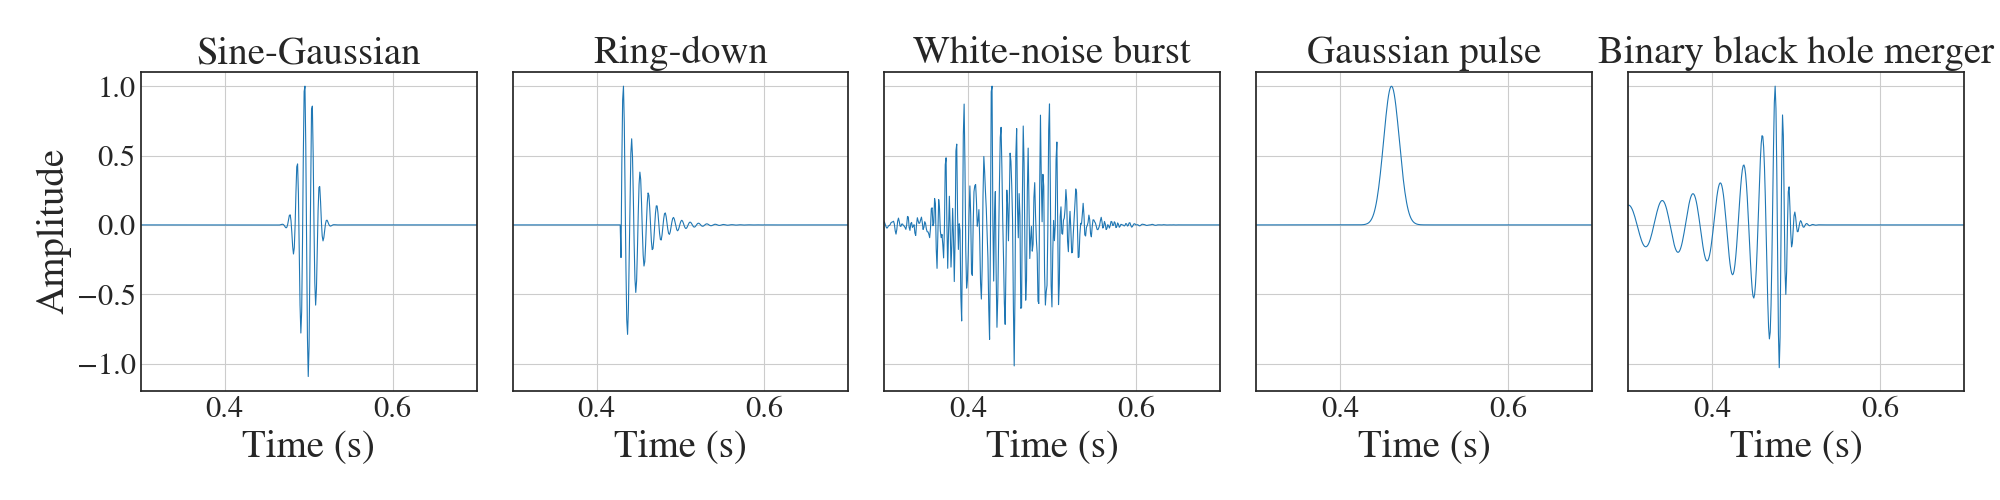
\includegraphics[width=\textwidth]{figures/training-sample.png}
    \caption{Examples of the five different waveforms that were used in training the \ac{GAN} for this study. Values of the parameters were selected randomly from uniform distributions from \cref{Tab:hyperparameters}.}
    \label{fig:training_waveforms}
\end{figure}

%%%%%%%%%%%%%%%%%%%%%%%%%%%%%%%%%%%%%%%%%%%%%%%%%%%%%%%%%%%%%%%%%%%%%%%%%%%%%%
\subsection{Architecture details}
%%%%%%%%%%%%%%%%%%%%%%%%%%%%%%%%%%%%%%%%%%%%%%%%%%%%%%%%%%%%%%%%%%%%%%%%%%%%%%
%
% Introduce some architecture features
%
For this work we use a \ac{DCGAN}~\cite{Radford2015} architecture. The generator model is fully convolutional,
upsampled using strided transposed convolutions
with batch normalisation in the
first layer and ReLU activations throughout with the exception of the Tanh activation for
the output layer. The use of Tanh guarantees the output function is bound between [-1,1]. Each transposed
convolutional layer uses a kernel size of 18 and stride of 2. The discriminator network
mirrors that of the generator without batch normalization, using
LeakyReLU activations, SpatialDropout, and a 2-stride convolution for
downsampling. The discriminator output is a single node with Sigmoid activation that can be interpreted as a probability of the the signal being real and both models are trained with binary cross
entropy. The full architecture description can be seen in~\cref{Tab:hyperparameters}.


% describe the hyperparameter tunings
%
Neural networks and subsequently \acp{GAN} have multiple parameters a developer
can tune when designing the model and these are referred to as hyperparameters.
The final network design used in this work comes from the use of trial and
error and the initial designs influenced by the available literature. We found
that the \ac{GAN} performed better with both networks having the same number of
layers and neurons which encourages even
competition between the generator and discriminator.  After tuning the multiple
hyperparameters (see \cref{Tab:hyperparameters}), the \ac{GAN} was trained on
$10^5$ signals  drawn from a categorical
distribution with equal propabilities for each class of
sine-Gaussian,
ring-down, white noise bursts, Gaussian pulse and \acp{BBH}. \jordan{add how many epochs trained for, on what hardware and how long}

As \acp{GAN} are trained by updating one model at the expense of the other, they can be hard to train. The goal of GAN training is to find an equilibrium between the two models, if this cannot be found then it is said that the \ac{GAN} has failed to converge. One way to diagnose \acp{GAN} during the development process is to keep track of the loss and accuracy over time. Loss plots, for example, as seen in \cref{fig:lossplot} can help to identify common failure modes or to check if the \ac{GAN} has indeed converged. Accuracy is the number of correct predictions made divided by total number of predictions. There is currently no notion of early stopping in \acp{GAN}, instead, training is halted after convergence and by visually inspecting the generations. 

\begin{figure}[h!]
    \centering
    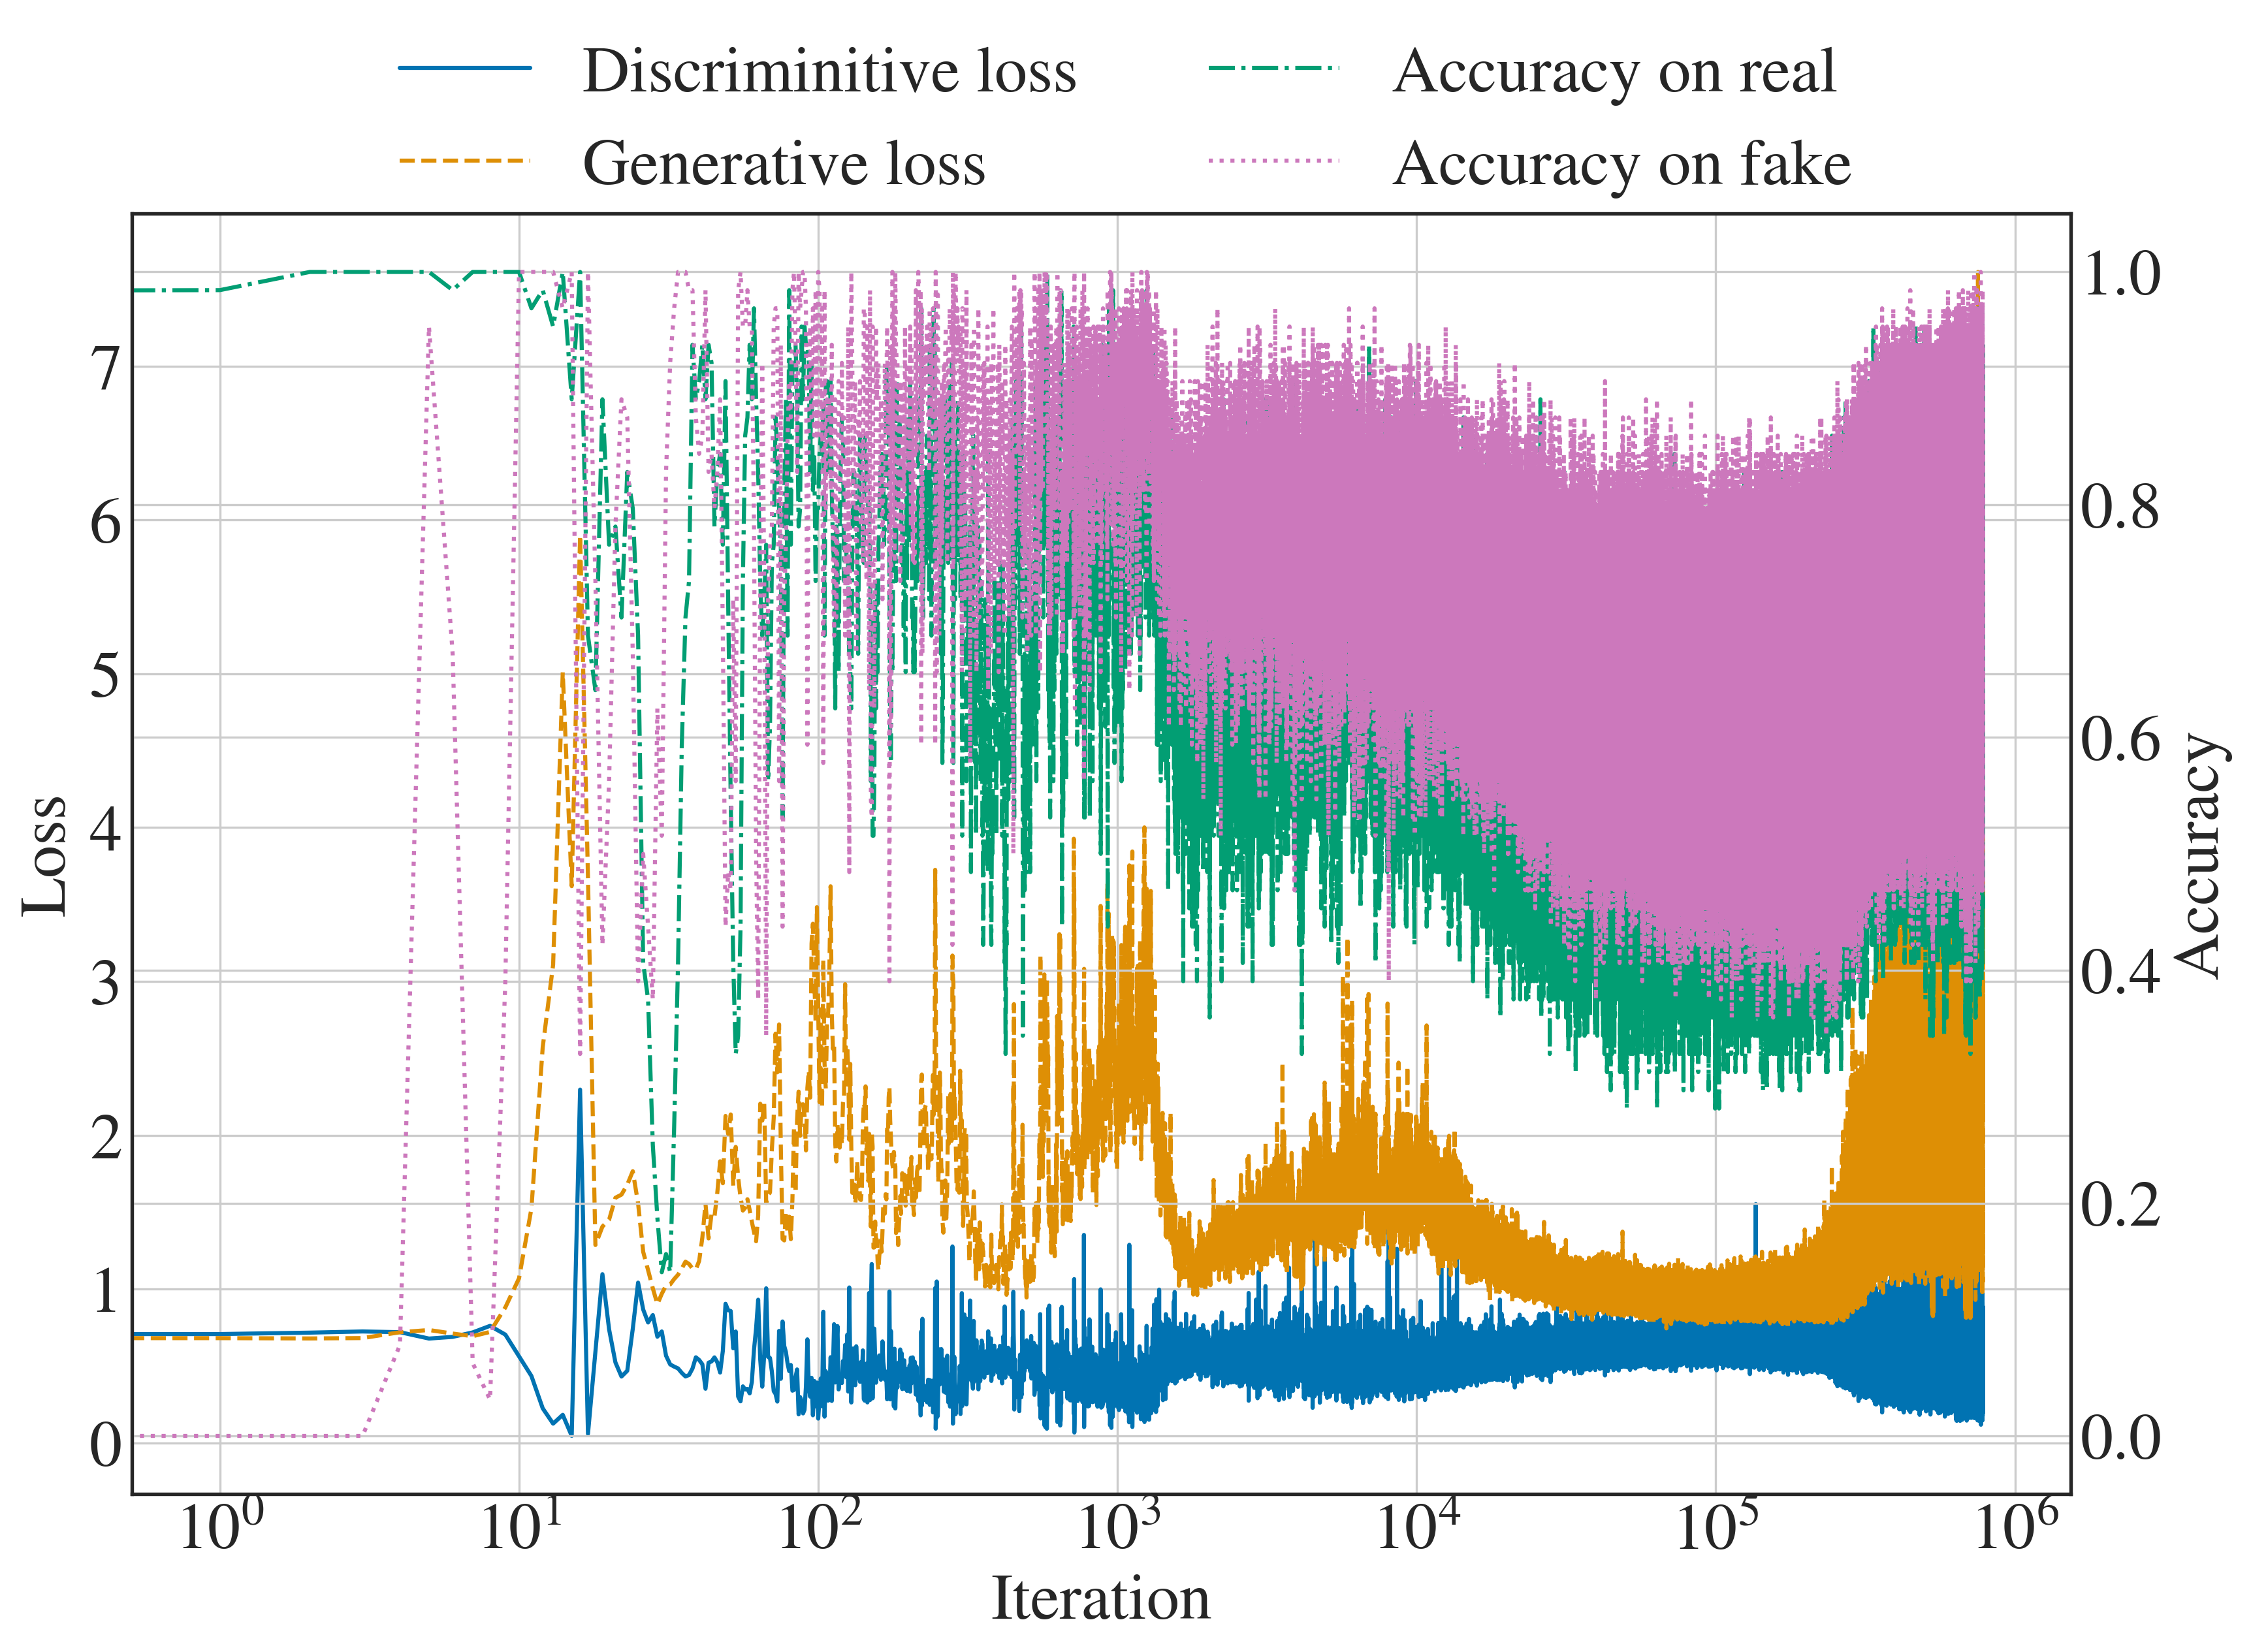
\includegraphics[width=1\textwidth]{figures/losses.png}
    \caption{Plot of the discriminator and generator loss and accuracy as a function of iterations. Early in training the losses oscillates as both models attempt to find their equilibrium, after which, both losses vary around a point which signifies stable training. Accuracy's on the real and fake data are similar showing that neither model is stronger than the other.}
    \label{fig:lossplot}
\end{figure}

%%%%%%%%%%%%%%%%%%%%%%%%%%%%%%%%%%%%%%%%%%%%%%%%%%%%%%%%%%%%%%%%%%%%%%%%%%%%%%
\section{Results}
%%%%%%%%%%%%%%%%%%%%%%%%%%%%%%%%%%%%%%%%%%%%%%%%%%%%%%%%%%%%%%%%%%%%%%%%%%%%%%


\begin{comment}
\begin{itemize}
\item Begin by outlining the type of results you will be presenting
\item A subsection on the general quality of generated waveforms - we may need
to have overlaps between generated wavefoms and training data (maybe)
\item A subsection on the descriminator - maybe a confusion matrix?
\item a subsection on the latent space varaition within each class - fixed
class, sliding in latent space.
\item A subsection on the class space variation - fixed latent space and
sliding in the class space.
\item A final subsection on the general waveform model based on random latent
and class space locations.
\item Make no conclusions.
\end{itemize}
\end{comment}

% describe the main idea
%
Given a 100-dimensional vector drawn from a normal distributed latent space and a one-hot encoded class
label, the GAN is able to generate burst-like waveforms generalised from the
training set. We set out by describing the quality of generated waveforms and
how they compare to the training set. We then explore the structure of the
latent and class spaces by interpolating between points in these spaces. We
test two methods of sampling from the class space that can be used to generate
a new breed of signal composed of weighted elements of each training class.


\begin{figure}
    \centering
    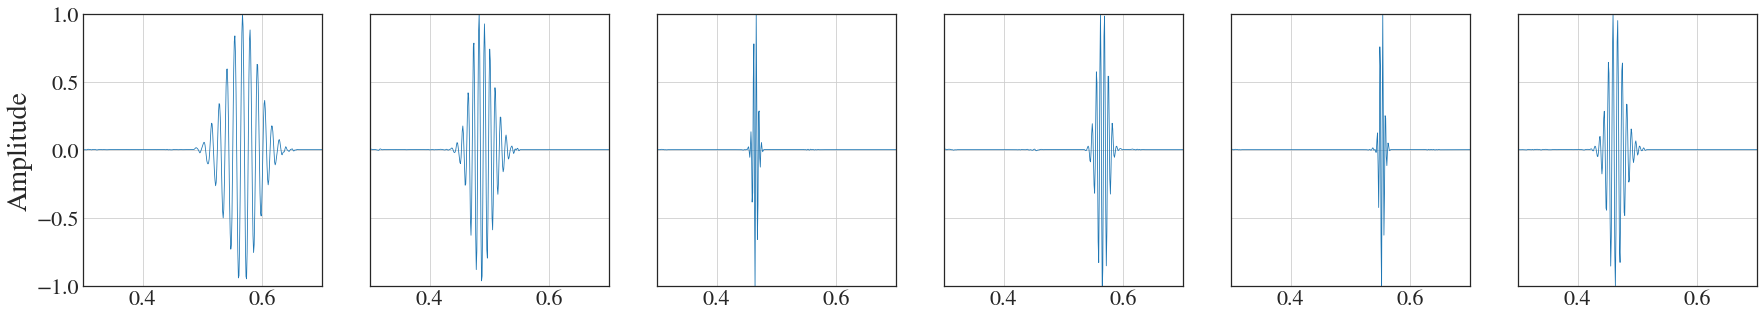
\includegraphics[width=\textwidth]{figures/generations/sg.png}
    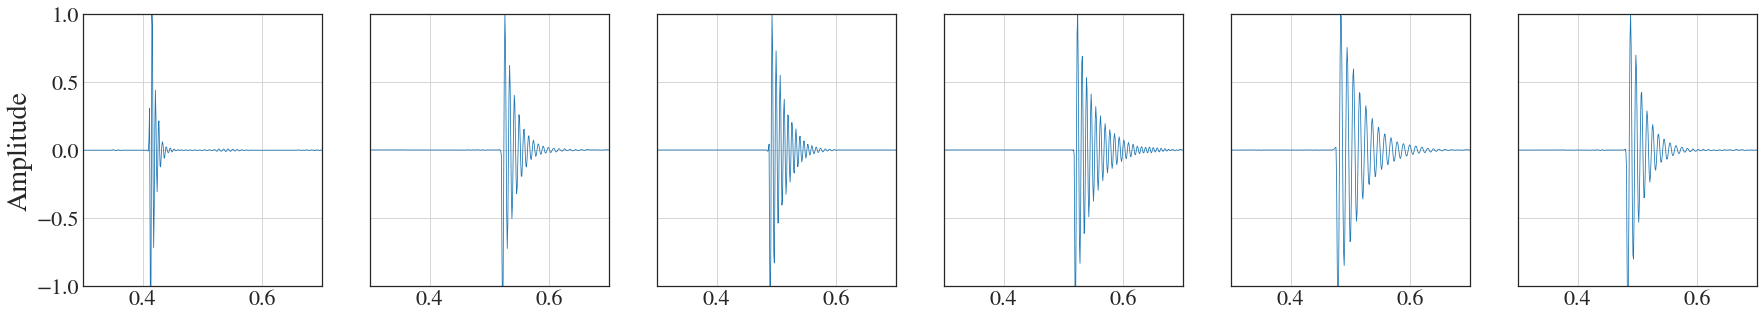
\includegraphics[width=\textwidth]{figures/generations/rd.png}
    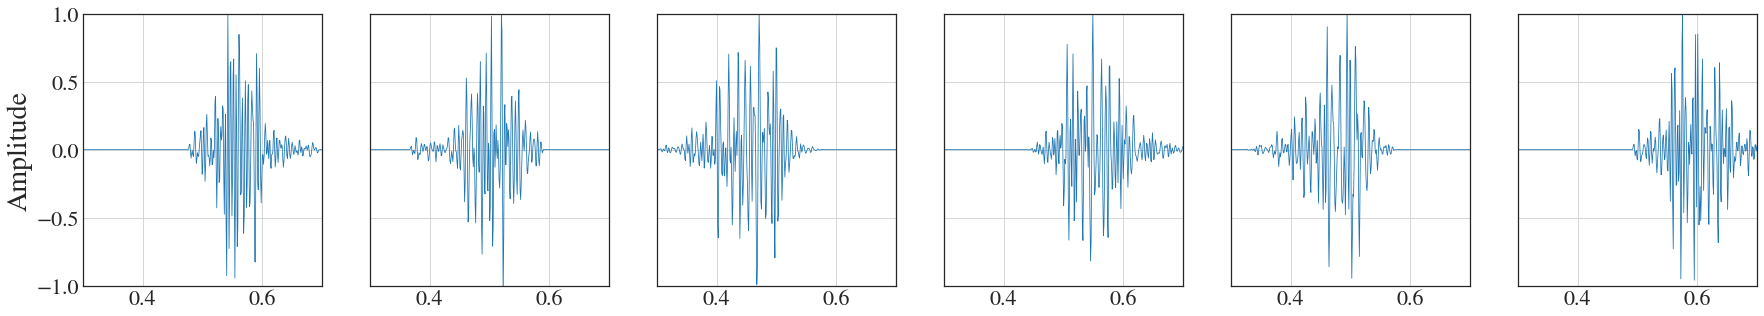
\includegraphics[width=\textwidth]{figures/generations/wnb.png}
    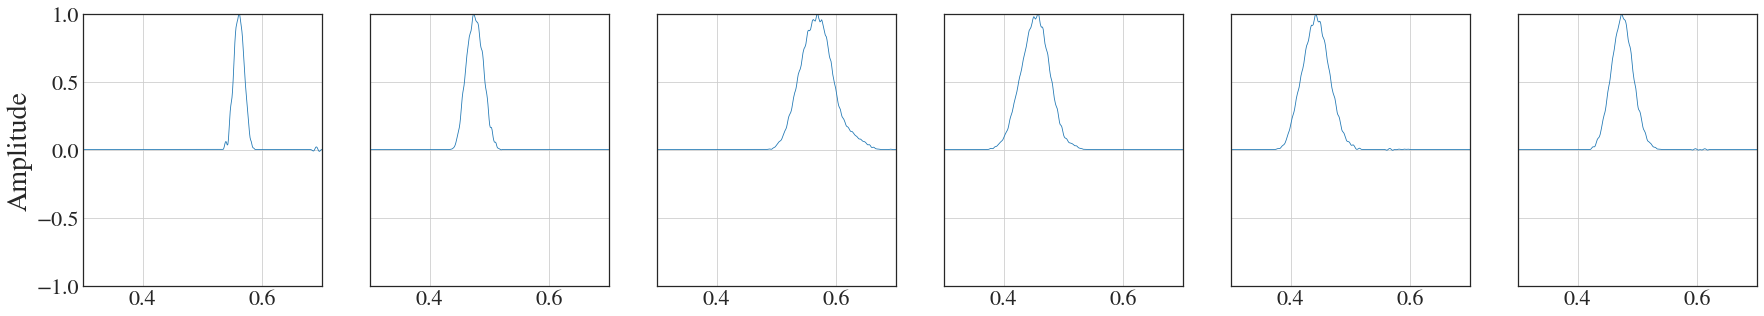
\includegraphics[width=\textwidth]{figures/generations/blip.png}
    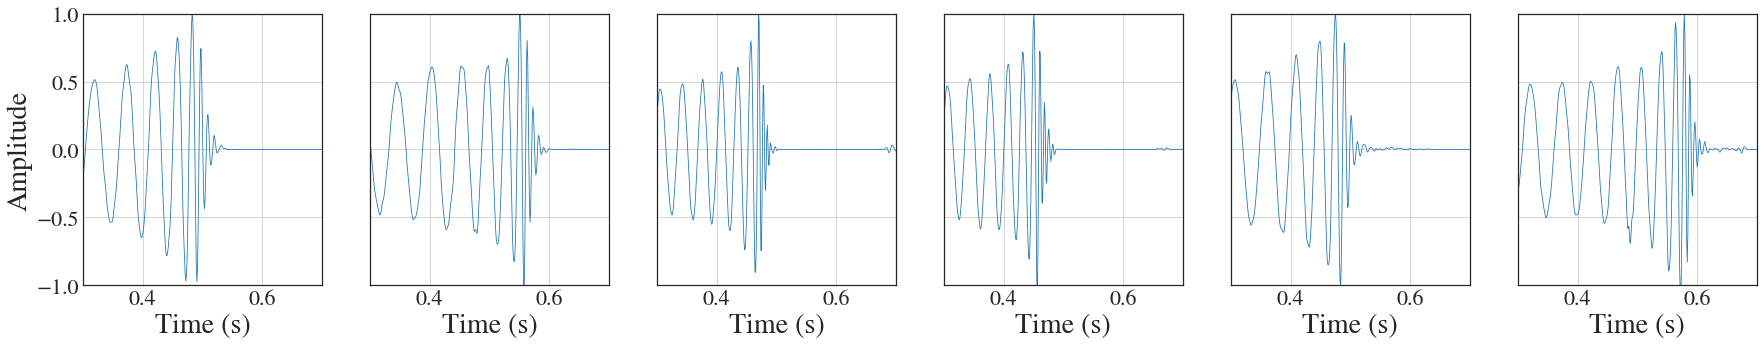
\includegraphics[width=\textwidth]{figures/generations/bbh.png}
    \caption{\ac{GAN} Generated waveforms plotted as a function of time. The latent space inputs for each panel is randomised and each row is assigned one of the five class vectors. By row: Sine-Gaussian, Ringdown,
White-noise burst, Gaussian pulse, Binary black hole merger. On the first four rows each x axis is zoomed for ease of viewing, while the last row shows the full one second.}
\label{fig:gen_signals} 
\end{figure}

%%%%%%%%%%%%%%%%%%%%%%%%%%%%%%%%%%%%%%%%%%%%%%%%%%%%%%%%%%%%%%%%%%%%%%%%%%%%%%
\subsection{Known class signal generation}

After training the networks, the generator's function is to map $G$ : $\mathbf{z},\mathbf{c} $ $\in$
$\mathbb{R}^{100}$ $\to$ $\mathbb{R}^{1024}$. The results from the
generator can be seen in \cref{fig:gen_signals}. Each plot shows the output of
the generator for random input latent space vectors $\mathbf{z}$ and each row
corresponds to one of the five class vectors $\mathbf{c}$. The generations show good quality likeliness and good variation within each class representative of the variation of the training data. All generations are single plus polarised waveforms and their amplitudes are normalised to unity after generation. 

%%%%%%%%%%%%%%%%%%%%%%%%%%%%%%%%%%%%%%%%%%%%%%%%%%%%%%%%%%%%%%%%%%%%%%%%%%%%%%
\subsection{Interpolation within the latent space}

% expain what we are planning to show here
%
\ac{ML} algorithms are often described as universal function approximators. In
the case of the generator it maps samples drawn from a 100 dimensional Gaussian
distribution in the latent space to its representation of the training set. As
with any function, there should be a one to one mapping from the domain and
co-domain to allow for smooth transitions across the latent space. Most GANs perform well on relatively low resolution
image generations, however, higher resolutions demand larger networks and long
training times. GANs attempting to replicate complicated structures and do not
have the necessary architecture either struggle to produce results at all or
fall into the common failure mode know as mode collapse; where the generator
produces a small variety of samples or simply memorises the training set. To
test this, we perform linear interpolations in the latent and class
space. We take two random
points in the 100-dimensional latent space and linearly interpolate between them. These new interpolated latent space vectors along with class vectors can now be fed into the generator to produce interpolated waveforms. \cref{fig:z_interp} shows the generated waveforms, with the class vectors held constant along each row. We can see that each plot shows plausible waveforms suggesting that
the generator has constructed a smooth traversable, space. Additionally, as each class is given
the same latent points to interpolate over, we can see that the waveforms
cluster together with respect to their parameters. Visually, the sine-Gaussian
and ring-down waveforms share similar frequencies and the other signals show
similar decays and starting epochs for a common latent space input. 
 
\begin{figure}
    \centering
    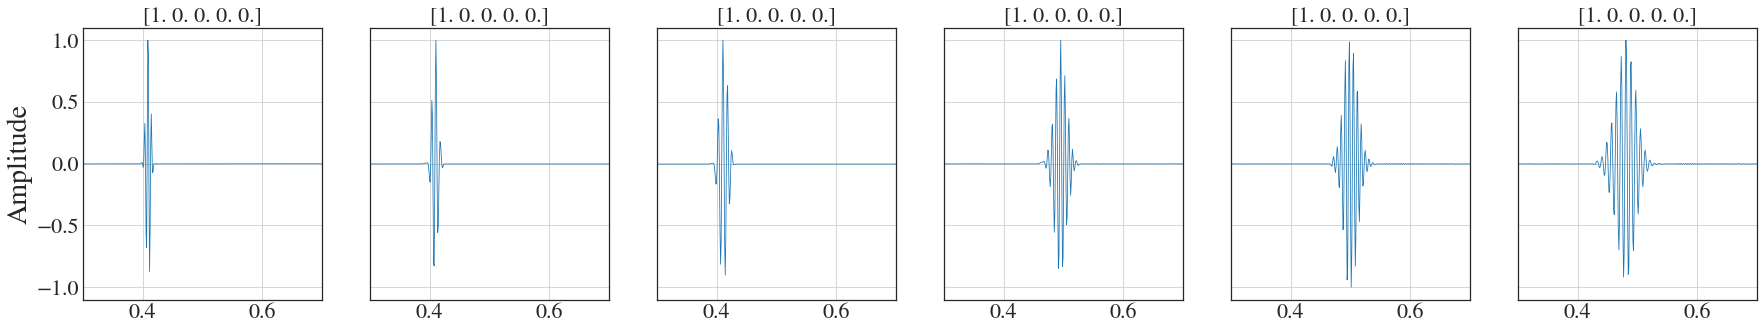
\includegraphics[width=\textwidth]{figures/generations/z_interp_sg.png}
    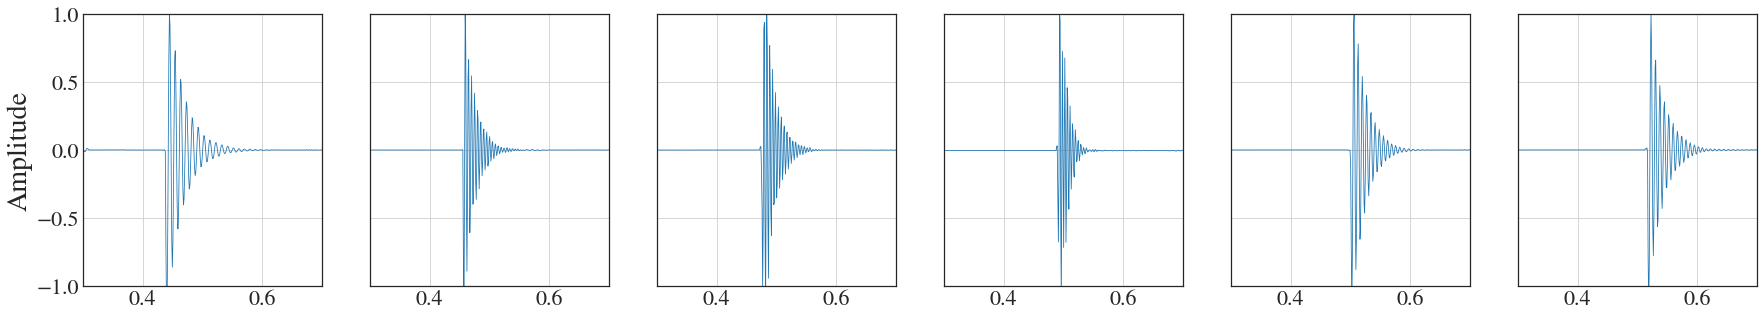
\includegraphics[width=\textwidth]{figures/generations/z_interp_rd.png}
    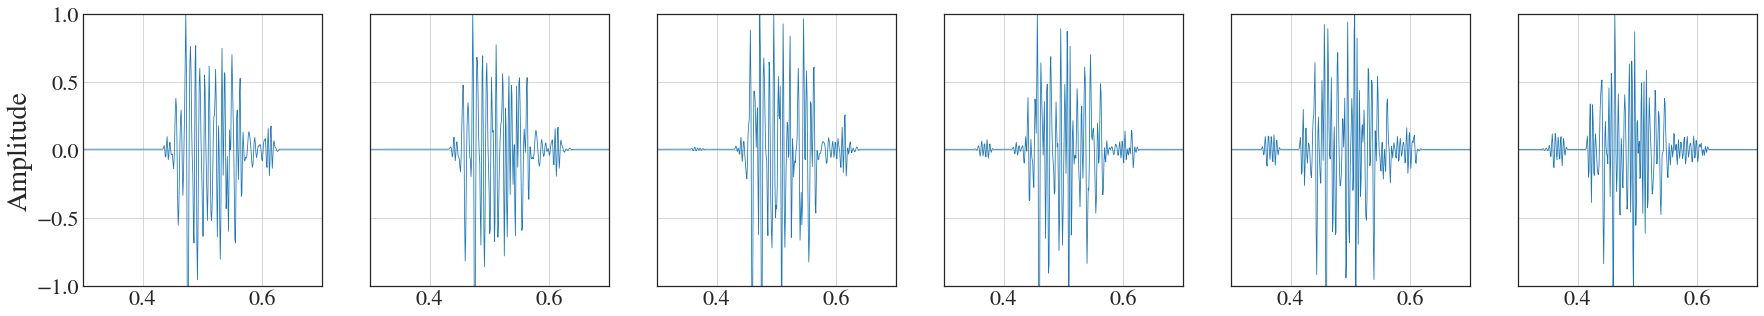
\includegraphics[width=\textwidth]{figures/generations/z_interp_wnb.png}
    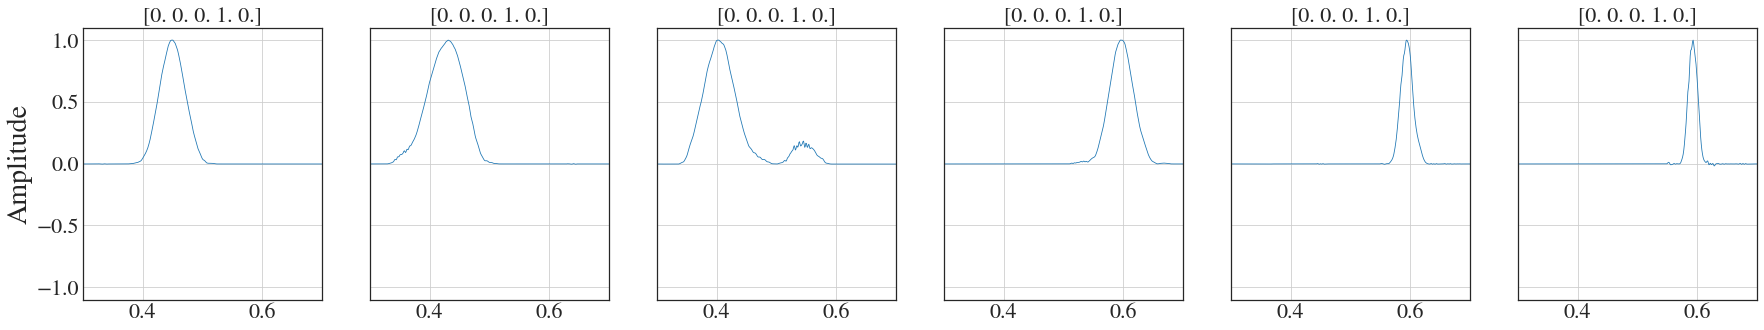
\includegraphics[width=\textwidth]{figures/generations/z_interp_blip.png}
    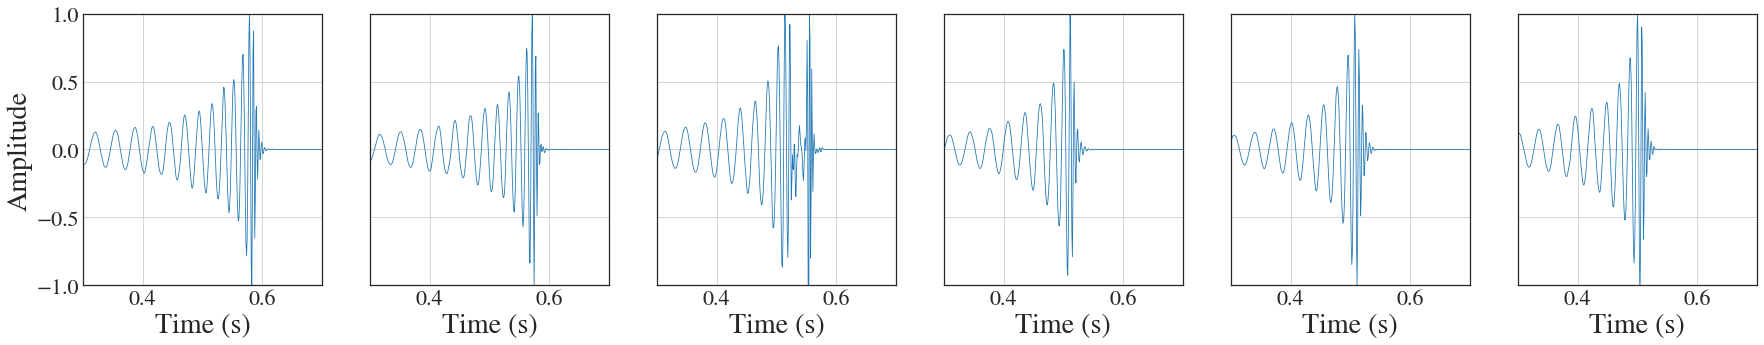
\includegraphics[width=\textwidth]{figures/generations/z_interp_bbh.png}
    \caption{Generated interpolated waveforms plotted as a function of time. The latent space inputs for the first  column is a vector of zeros and last columns are vectors of 0.5. Between panels are linearly interpolated vectors between these two points. Each row keeps on of the class vetors constant thoughout the latent space interpolation. On the first four rows each x axis is zoomed for ease of viewing, while the last row shows the full one second time interval.}
    \label{fig:z_interp}
\end{figure}

%%%%%%%%%%%%%%%%%%%%%%%%%%%%%%%%%%%%%%%%%%%%%%%%%%%%%%%%%%%%%%%%%%%%%%%%%%%%%%
\subsubsection{Interpolation between pairs of classes}

While the \ac{GAN} is trained on distinct one-hot encoded classes, we may test arbitrary points in the 5-dimensional space to produce indistinct or "inbetween" waveforms. In order to explore the class space we keep the latent vector constant and
interpolate through the 5 classes. We construct a path between two waveforms
and show in \cref{fig:c_in	terp} that the space is populated enough to allow for transitions between
classes.  Sine-Gaussian to ringdown performs well in interpolation with each
signal being a plausible burst GW. It is obvious that the GAN has clustered
these two groups during training as they share many characteristics. The other
signals have sharper transitions but still retain plausible looking waveforms. 

\begin{figure}
    \centering
    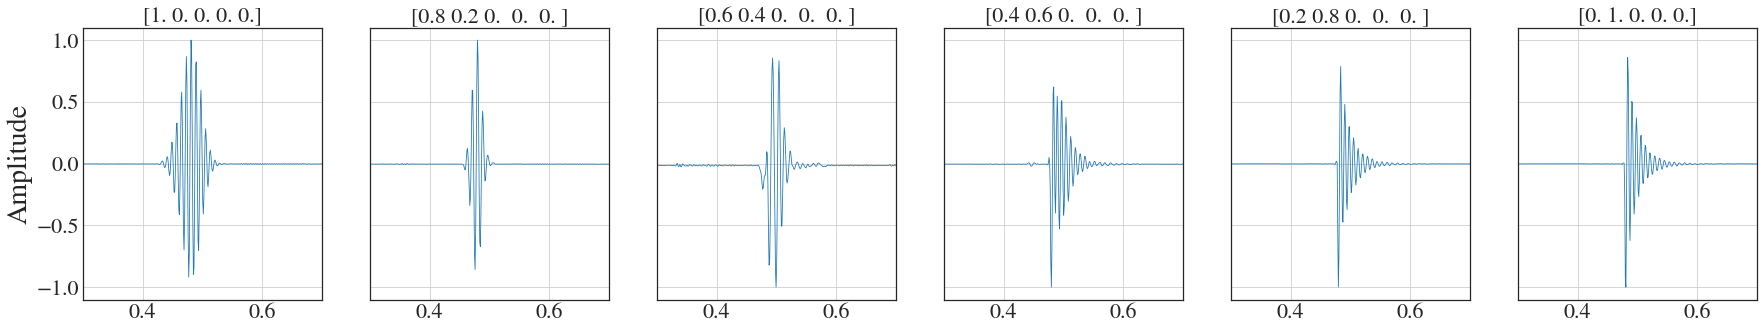
\includegraphics[width=\textwidth]{figures/generations/sg-rd.png}
    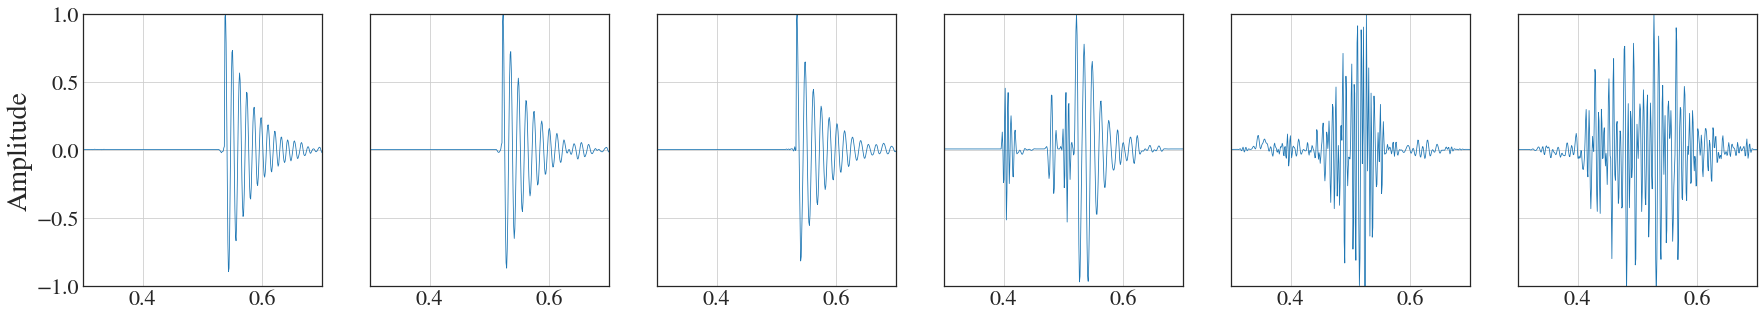
\includegraphics[width=\textwidth]{figures/generations/rd-wnb.png}
    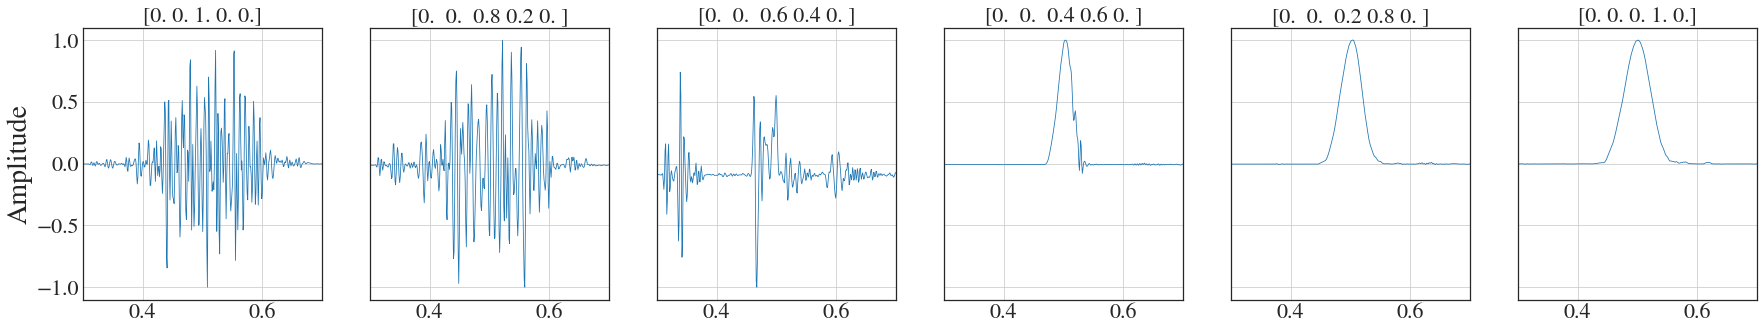
\includegraphics[width=\textwidth]{figures/generations/wnb-blip.png}
    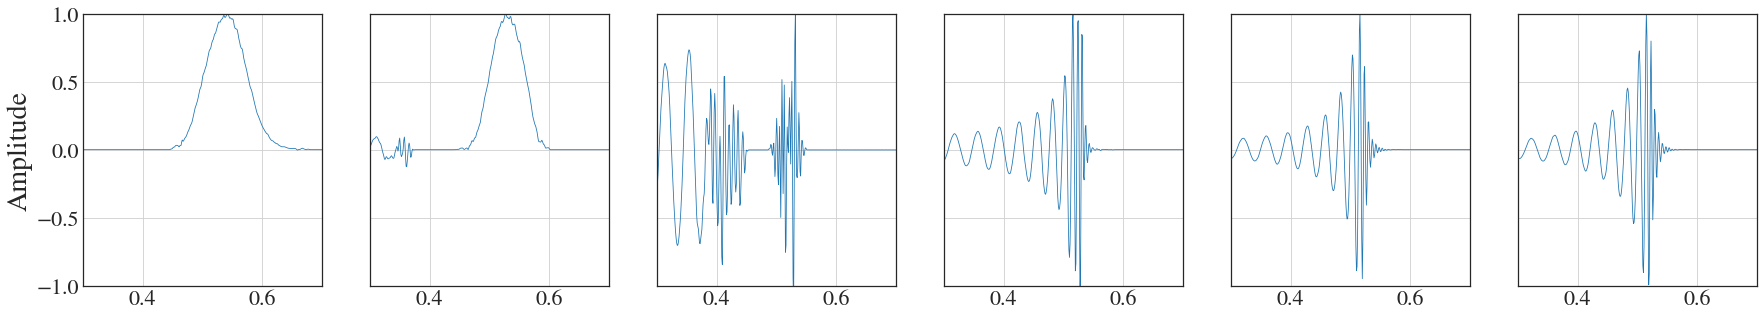
\includegraphics[width=\textwidth]{figures/generations/blip-bbh.png}
    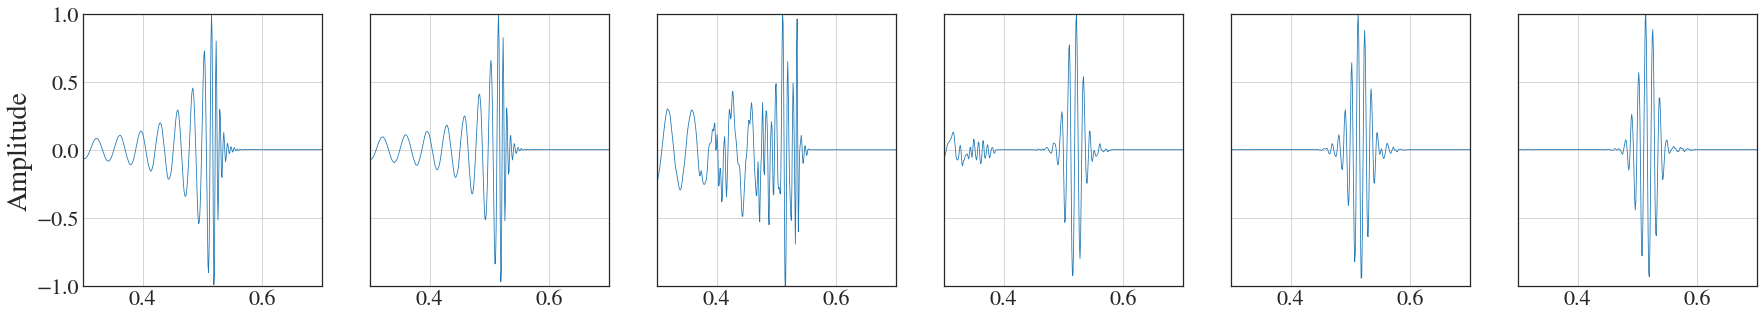
\includegraphics[width=\textwidth]{figures/generations/bbh-sg.png}
    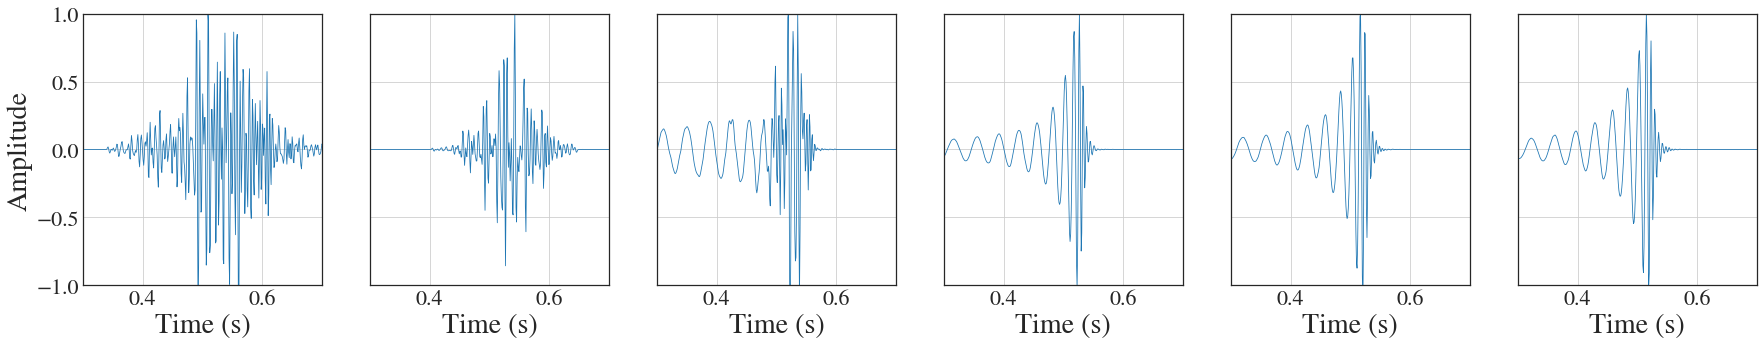
\includegraphics[width=\textwidth]{figures/generations/wnb-bbh.png}
    \caption{Generated class interpolated waveforms as a function of time. The latent space vectors are fixed at 0.5 for each entry while each row shows generations using linearly interpolated classes as inputs to the generator. By row top to bottom: Sine-Gaussian to Ringdown, Ringdown to White-noise burst, Gaussian pulse to BBH, BBH to Sine-Gaussian, White-noise burst to BBH.}
    \label{fig:c_interp}
\end{figure}

\subsection{General points within the class space}
We have shown that the \acp{GAN} latent space and class space has structure that can be navigated through with interpolation between paris of signals. Taken a step further, we can sample from the class space in novel ways to create new inputs for the generator. These new points are categorised by the method used to sample from the class space. The methods we use are divided into the following: 

\begin{itemize}
%
\item {\bf Vertex}: Points that lie at the corners of the five dimensional class space.
These signals are the closest to the training set.
%
\item {\bf Uniform}: Generated using a uniform distribution U[0,1] as the input
class vector.
%
\item {\bf Simplex}: Generated using a Dirichlet distribution that samples from the
4-simplex inside the class space.
%
\end{itemize}

The vertex points are the most straightforward where one entry contains 1 and the other entries are zero and are equivalent to the class vectors that the GAN is trained on e.g. $\mathbf{c} = [1,0,0,0,0]$ would correspond to a Sine-Gaussian generation. Uniform class vectors sample from a uniform distribution and act like a random draw from the class space. Uniformly sampling contains points up to a distance of unit from the closest class e.g. [0,0,0,0,0] is of distance 1 away from all classes (as is [1,1,1,1,1]). For simplex class vectors, we sample from the simplest hypersurface that intersects all the classes and has a symmetry such that no class is favoured over any other. For our 5-dimensional case this would correspond to a 4-simplex manifold. Sampling from the simplex can be seen as sampling from between the classes within the space. We can expect a priori that the uniformly sampled space (which contains the simplex as a subspace) will allow for some level of extrapolation. 

~\chris{Also, discuss the corresponding figure! There has to be comment on the
features of simplex vs box generations as well as general comments about how
the GAN likes to mix signals up. Pick on specific examples and comment on
interesting or annoying features.}

\begin{figure}
    \centering
    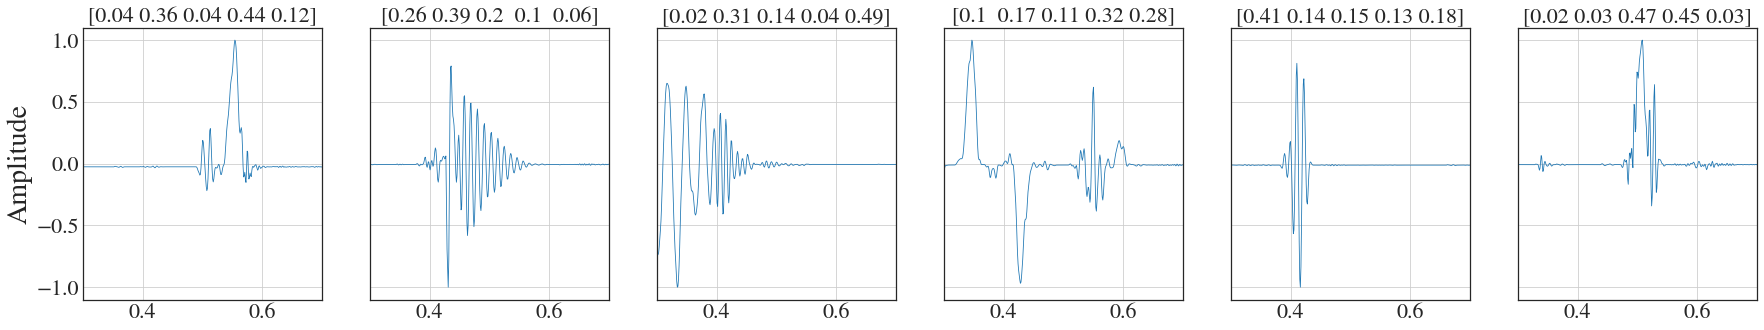
\includegraphics[width=\textwidth]{figures/generations/simplex_sample1.png}
    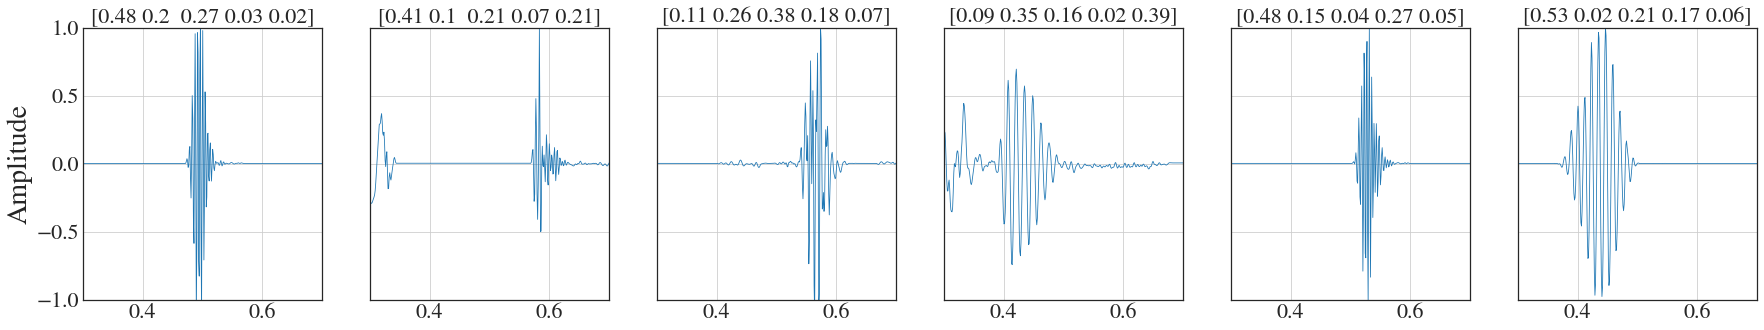
\includegraphics[width=\textwidth]{figures/generations/simplex_sample2.png}
    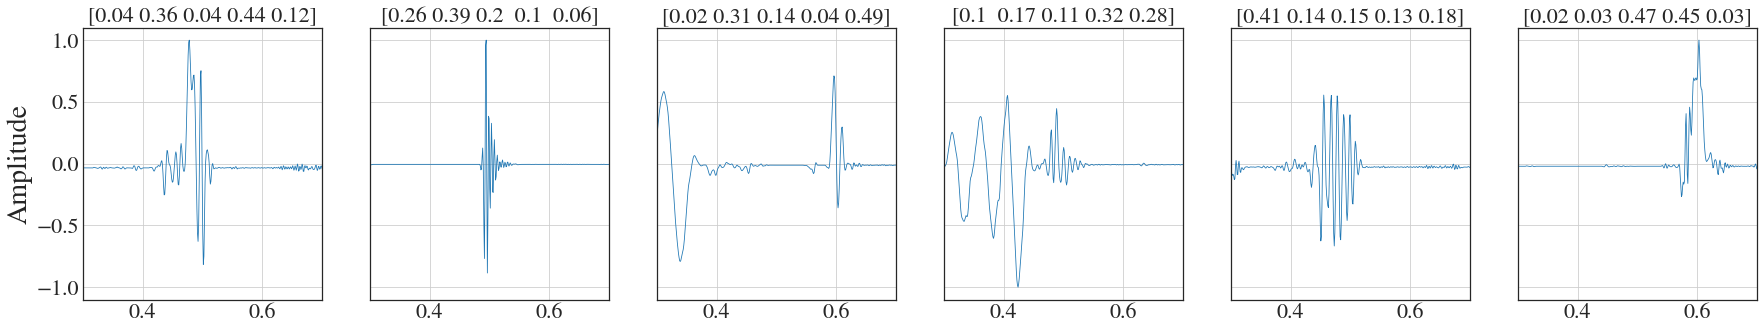
\includegraphics[width=\textwidth]{figures/generations/simplex_sample3.png}
    \caption{GAN generations where the class vectors are sampled from the 4-D
plane intersecting all classes. Latent space locations for all signals are taken randomly from a Gaussian distribution and the signals are then re-scaled such that they peak at unity.}
    \label{fig:simplexd_samples}
\end{figure}

\begin{figure}
    \centering
    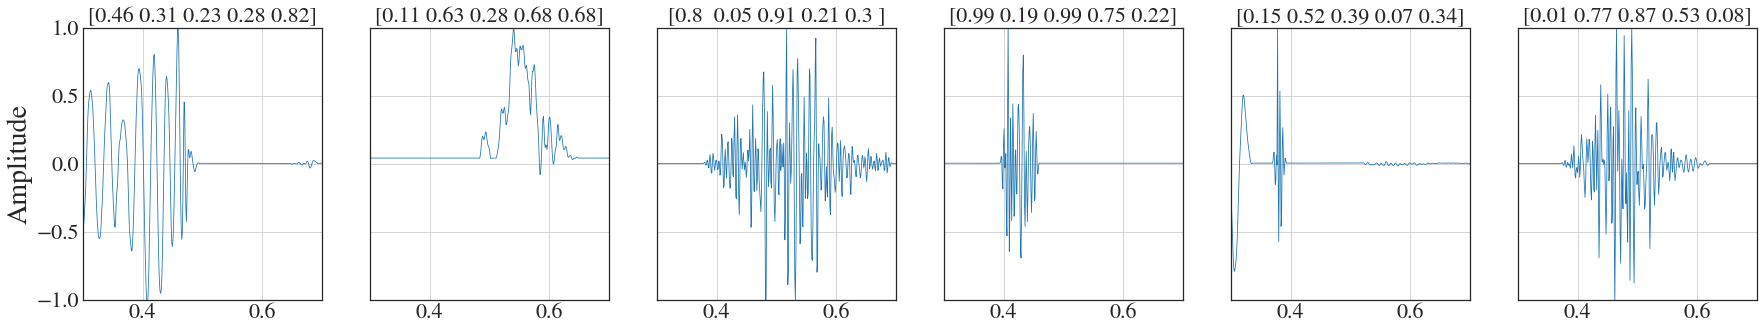
\includegraphics[width=\textwidth]{figures/generations/uniform_sample3.png}
    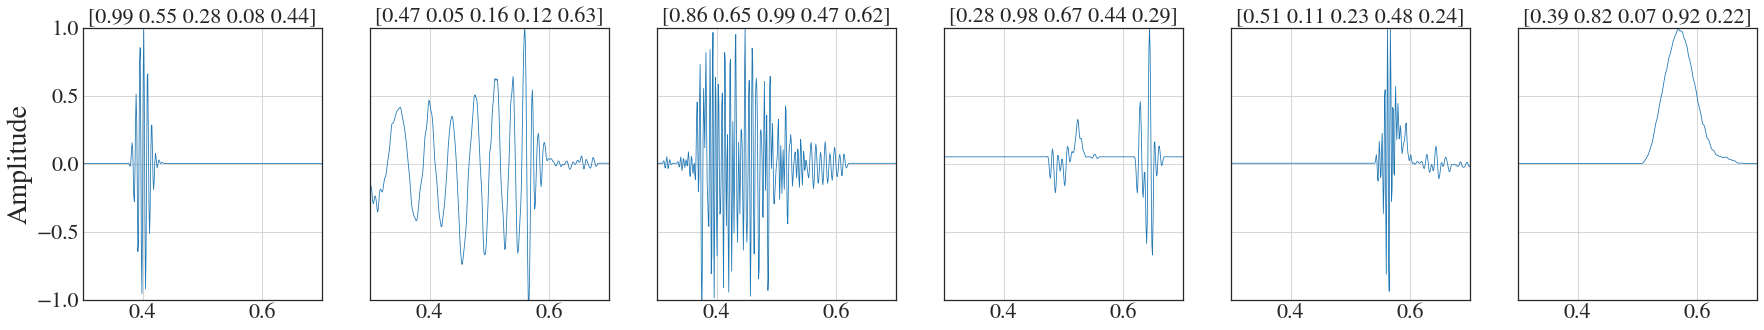
\includegraphics[width=\textwidth]{figures/generations/uniform_sample2.png}
    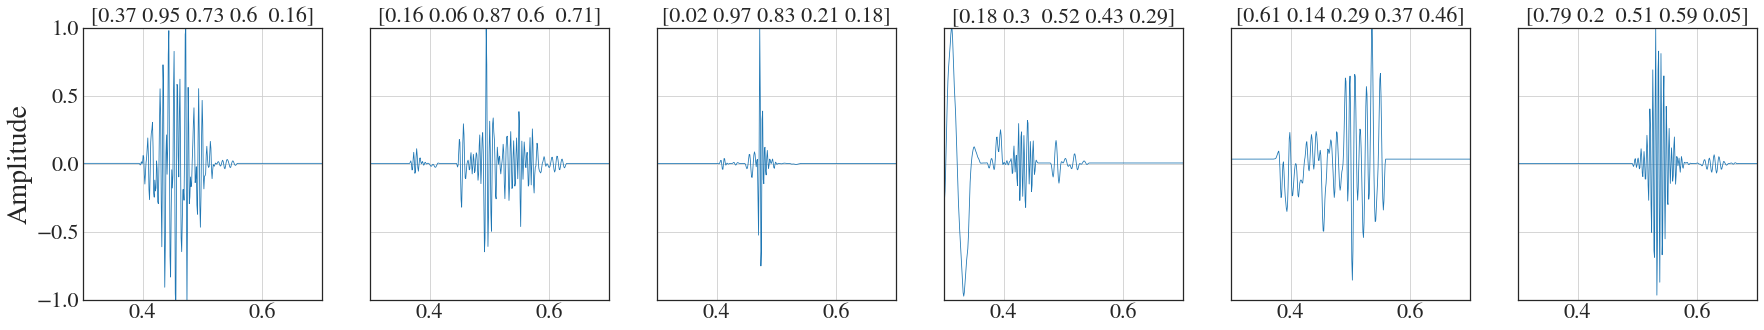
\includegraphics[width=\textwidth]{figures/generations/uniform_sample1.png}
    \caption{GAN generations where the class vectors are sampled uniformly in the hypercube class space. Latent space locations for all signals are taken randomly from a Gaussian distribution and the signals are then re-scaled such that they peak at unity.}
    \label{fig:uniform_samples}
\end{figure}

~\chris{I have an idea for the plots. Could we have a colour coding system
where each class gets a colour and then when you mix them you plot it with the
mixed colours - you average the RGB values. Maybe everything would look brown?
Worth a try?}

\section{Searching for generalised burst using a CNN}
In this section  we use a convolutional neural network \ac{CNN} 
to compare different waveform generations from the \ac{CGAN} to help determine the
success and failures of the model generations. We train a \ac{CNN} to distinguish between two classes: signals in additive Gaussian
noise and Gaussian noise only. 
\subsection{Training data} 
We use three classes of training data: Vertex, Uniform or Simplex cases generated using our \ac{GAN} method and consider two detectors H1 and L1 as joint inputs to the \ac{CNN}. For each training set we generated a bank of $2\times 10^5$ signals and apply antenna responses and time delays using routines provided by LALsuite \cite{lalsuite}. The polarisation angles are drawn uniformly in the range [0,2$\pi$] and sky positions are generated uniformly on the 2-sphere. Time delays between detectors are computed relative to the Earth centre. All of the training data used is whitened using the Advanced LIGO
design sensitivity \ac{PSD}, such that there is equal noise power at each
frequency and the data is correctly normalised. This procedure is
applied to signals whose \acp{SNR} are sampled uniformly in the range $[1-16]$. Each time series input to the \ac{CNN} is represented by an 1024 x 2 image that is sampled at 1024 hz for each of the two detectors. An example time series is shown in \cref{fig:cnn_training}. While training the network, the input training data consists of
signals which contain one half noise only and one half signal contained in
noise. Of that, 80\% is used for training and 20\% used for validation, while for testing we use $2\times 10^5$ signals in order to use small false alarm rates later.

\begin{figure}[ht!]
    \centering
    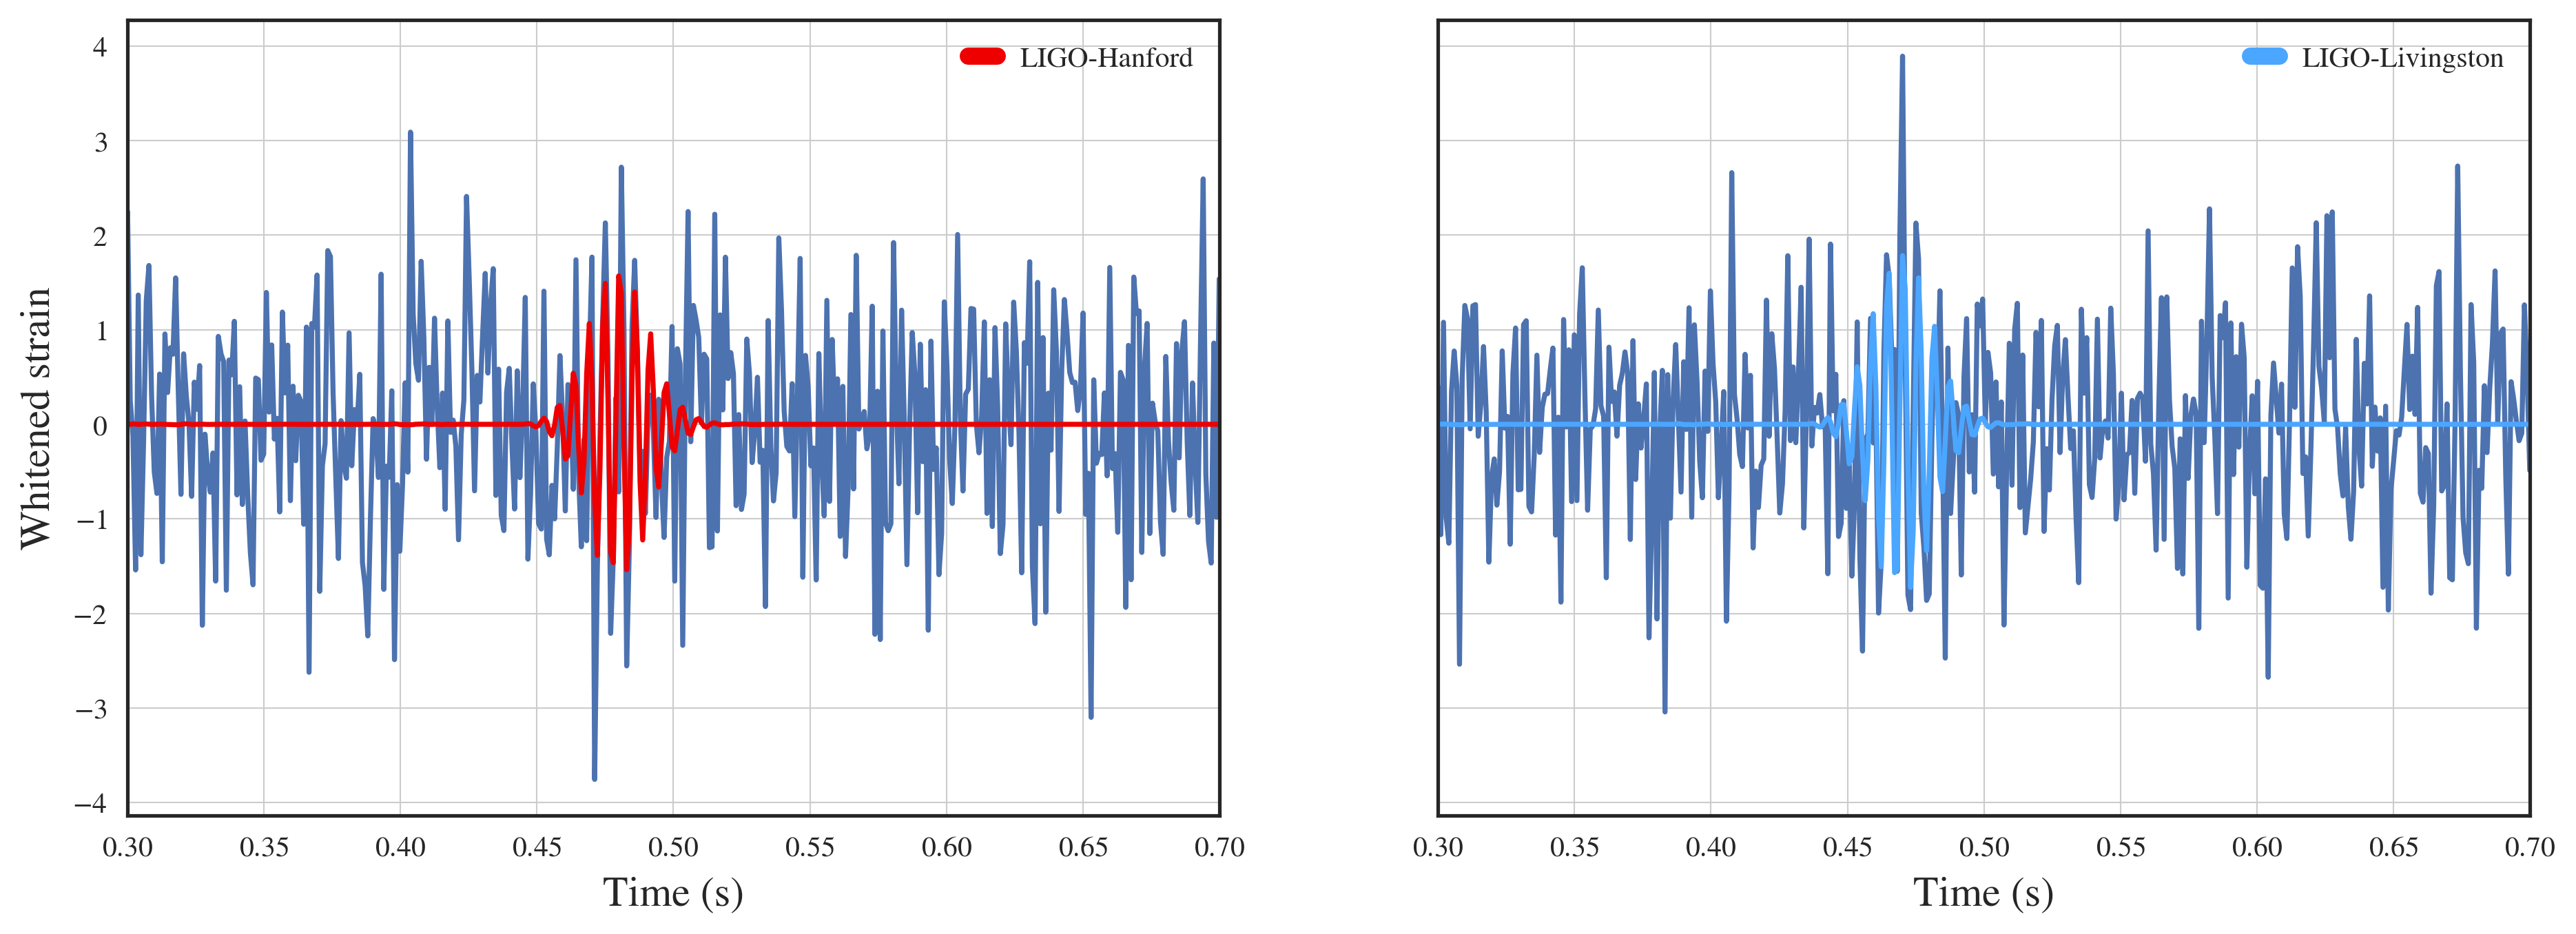
\includegraphics[width=\textwidth]{figures/SNR8.png}
    \caption{\ac{CNN} training data. Whitened noise free sine-Gaussian timeseries as seen by Hanford (red) and Livingston (light blue) detectors. These signals with fixed SNR = 8, re-scaled by the two detector network SNR. The dark blue time series for each plot shows either the same signal with added detector noise from Hanford (left) or Livingston (right). The signals plus added noise is used to train, test and validate the \ac{CNN}.}
     \label{fig:cnn_training}
\end{figure}

\subsection{CNN architecture}
In this approach the input to the \ac{CNN} is a two dimensional vector which is passed through a series of convolutional layers, onto two fully connected or ''Dense" layers and finally to a single output neuron which represents the probability that a signal is present within the noise. We used a small amount of dropout and found that the swish activation \cite{ramachandran2017searching} function performed well. The output layer is activated by a sigmoid function and we used \cref{eqn:crossentropy} as a loss function and Adam as an optimizer with learning rate set to $10^{-3}$. In total we train three separate \acp{CNN} on either the vertex, uniform or simplex data set, however, all \acp{CNN} share the same architectural
structure and hyperparameters which are shown in \cref{Tab:cnn_training_parms}.

In~\cref{fig:roc_curves} we compare the \ac{CNN} results between the three
datasets, we train three \acp{CNN} on the Conditional, simplex and uniform data sets
and use these models to make predictions on the other unseen datasets. We make
a comparison by fixing the fraction of samples incorrectly identified as
signals (false alarm rate) and plotting this versus the optimal SNR of the
signals.~\chris{this last sentence isn't quite right} 

\begin{figure}
    \centering
    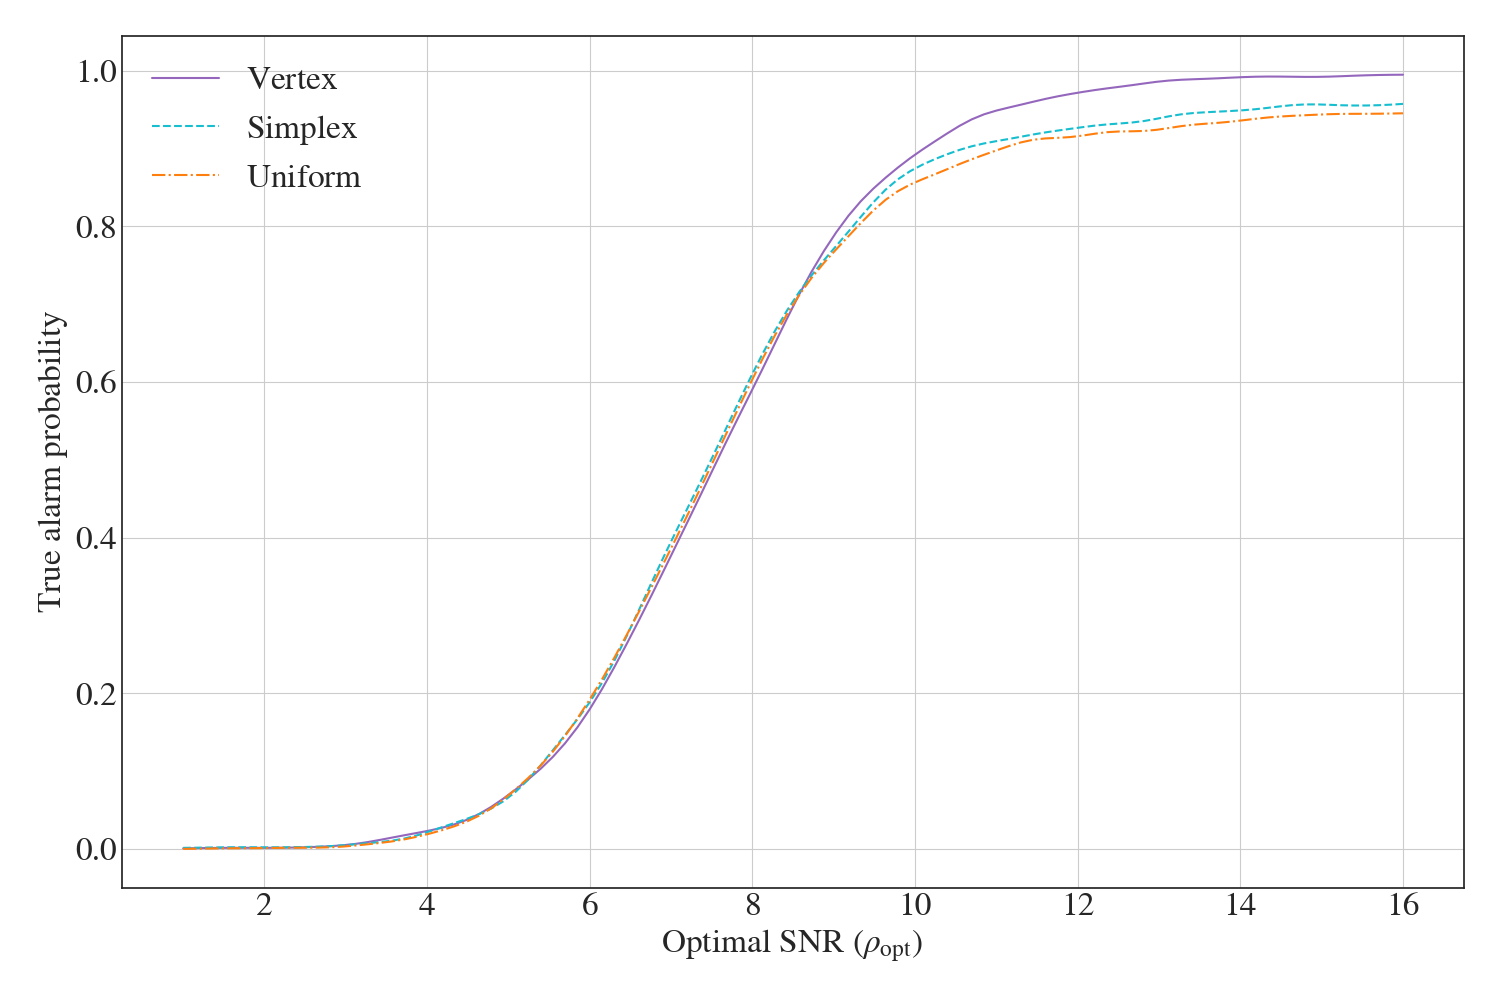
\includegraphics[width=0.8\textwidth]{figures/conditional_trained.png}
    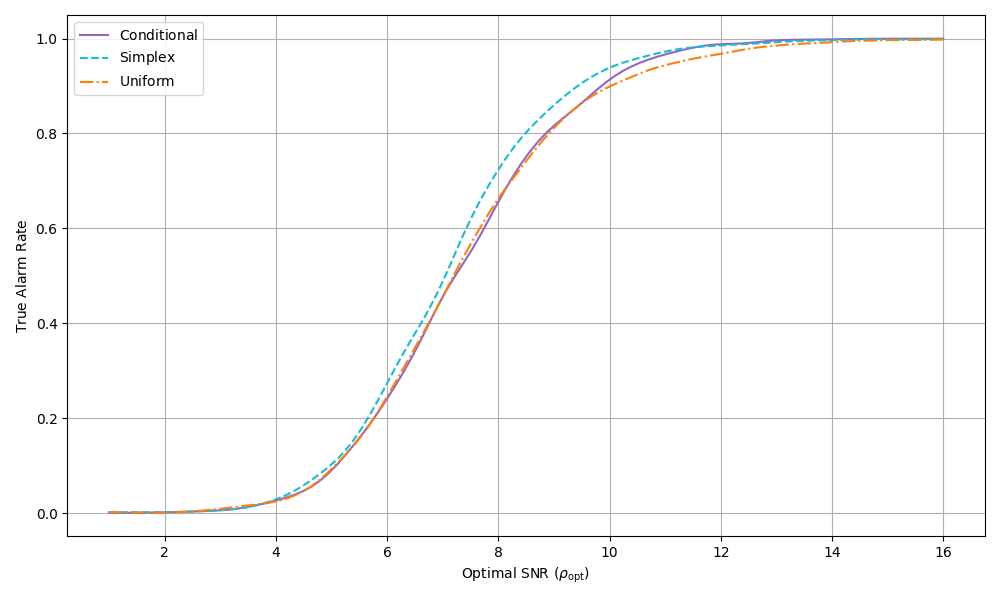
\includegraphics[width=0.8\textwidth]{figures/simplex_trained.png}
    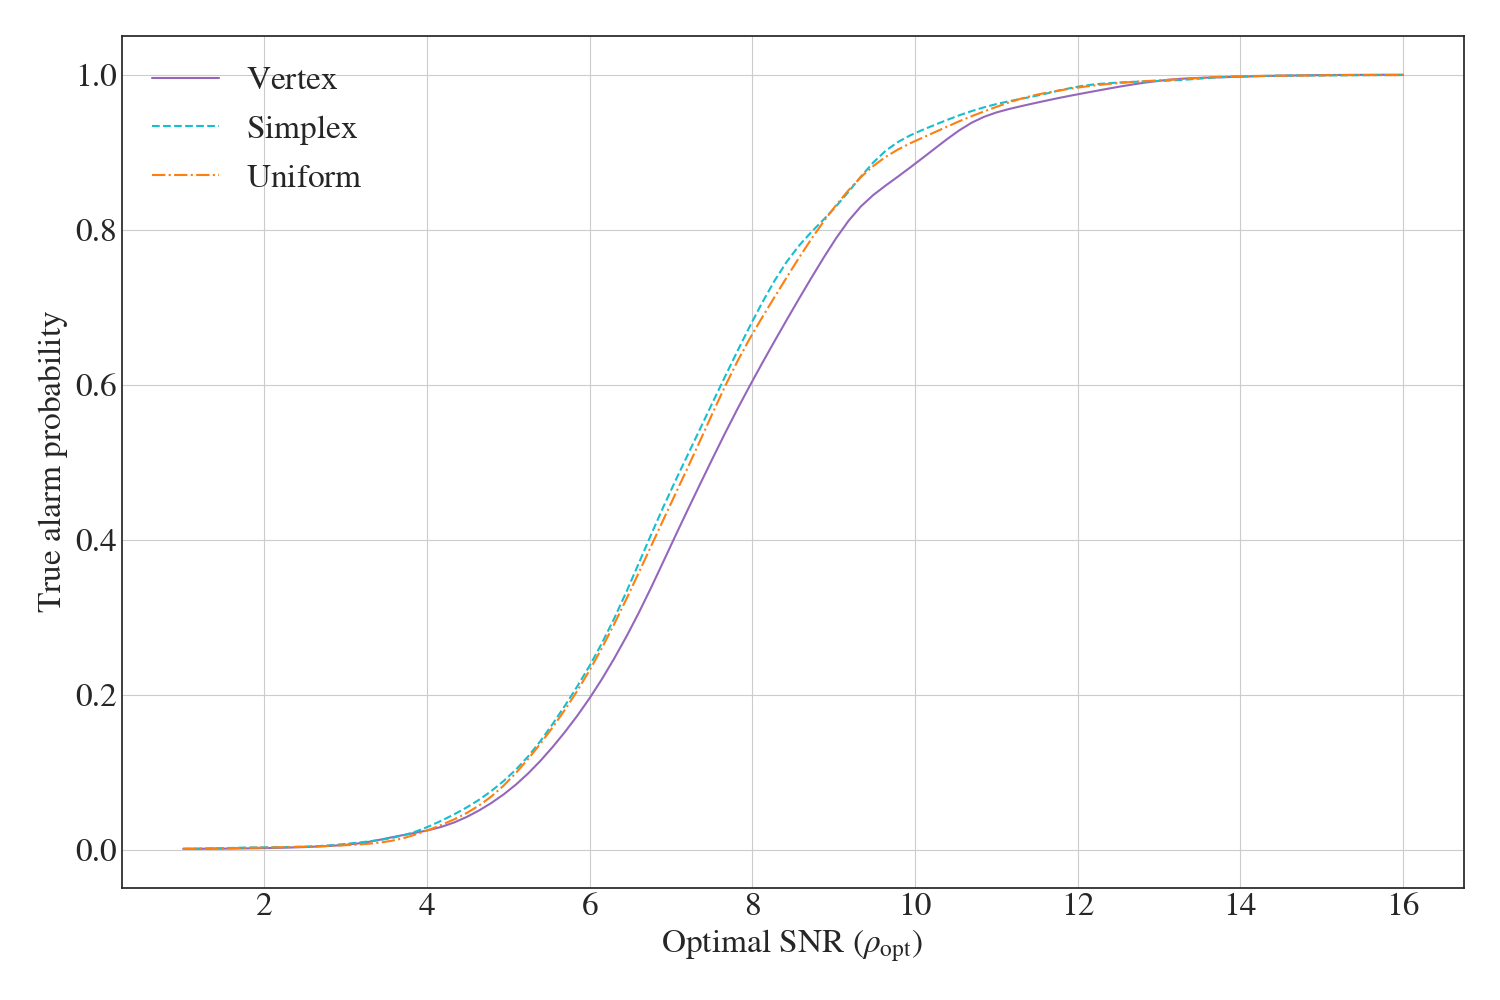
\includegraphics[width=0.8\textwidth]{figures/uniform_trained.png}
    \caption{Efficiency curves comparing the performance of \acp{CNN} trained on
conditional generations (top), simplex generations (middle), uniform
generations (bottom) for a fixed false alarm rate of $10^{-3}$.~\chris{more
description. What is plotted against what? The fonts are different to the other
plots. The y-axis is not a rate but a prbability (a FAP unfortunately)}}
\label{fig:roc_curves} 
\end{figure}

These results show for a \ac{CNN} trained on conditional signals, the uniform data
set is distinguishable from the conditional and simplex dataset. The \ac{CNN} is
robust enough to capture the differences between the datasets and shows that
the GAN can generate a variety of unmodelled waveforms that can be used in
future testing. 

~\chris{please write more about the results of the CNN}


%%%%%%%%%%%%%%%%%%%%%%%%%%%%%%%%%%%%%%%%%%%%%%%%%%%%%%%%%%%%%%%%%%%%%%%%%%%%%%
\section{Conclusions}
%%%%%%%%%%%%%%%%%%%%%%%%%%%%%%%%%%%%%%%%%%%%%%%%%%%%%%%%%%%%%%%%%%%%%%%%%%%%%%

% summary of the paper
%
In this work we present the potential of \acp{GAN} for
burst \ac{GW} analysis. We have shown that \acp{GAN} have the ability to generate realisitc time series burst data and can be conditioned based on the inherent features of the signals. The latent and class spaces were explored through interpolation and
suggest that the space provides smooth translations between classes and overall
waveform shape. We then showed targeted waveform generation by mixing classes
to produce new unmodelled waveform varieties that can be used to test current
burst search pipelines.

% extra things to think about
%

Having the ability to quickly
generate new waveforms is essential to test current detection schemes and their
susceptibilty to unmodelled sources. We believe that \acp{GAN} have the ability
to generate high fidelity waveforms at a fraction of the computational
expense~\chris{don't focus on the expense part since burst waveforms are cheap
anyway} and do not rely on large prior parameter space. Having banks of these
waveforms at hand can aid in our understand of the physics processes behind
these non-standard ac{GW} emitters.  
~\chris{we need to write down paragrph headinsg in the next meeting. I'm tired.}

\begin{comment}
\begin{itemize}
\item Summarise the paper
\item Dedicate a paragraph to each of the key results discussed in the previous
section
\item Have at least one paragraph on the future directions of this work
\item Conclude with a positive paragrpah about the potential uses and impact of
the approach.
\end{itemize}
\end{comment}

\section*{References}
\bibliography{references}

\clearpage

\appendix
\section{List of hyperparameters}
\begin{table}[hb]
\centering
\caption{The architecture and hyperparameters describing our CNN consists of four convolutional layers followed by two dense layers. The convolutional layers are activated by the swish function, the first dense layer is not activated and dropout is applied, while the final layer uses the sigmoid activation. The network is trained by minimising the binary cross entropy and optimised with Adam with learning rate $10^{-3}$. We train for 10 epochs with a batch size of 1000.}
%\footnotesize
\begin{tabular*}{\textwidth}{c @{\extracolsep{\fill}} c c c c c c}
\br
%\hline
Operation & Output shape & Kernel size & Stride & Dropout & Activation \\
\mr
Input & (1024, 2) & N/A  & N/A & N/A & N/A \\
Convolutional & (512, 8) & 5 & 2 & 0 & Swish  \\
Convolutional & (256, 8) & 5 & 2 & 0 & Swish  \\
Convolutional & (128, 8) & 5 & 2 & 0 & Swish  \\
Convolutional & (64, 8) & 5 & 2 & 0 & Swish  \\
Dense & (100) & 100 & N/A & 0.2 & Linear  \\
Dense & (1) & 1 & N/A & 0 & Sigmoid \\
\end{tabular*}\\
\begin{tabular*}{\textwidth}{@{}l l l l l l}
\mr
Optimizer & Adam($\alpha$ = 0.001, $\beta_{1}$ = 0.5) & & & & \\
Batch size & 1000 & & & & \\
Epochs & 100 & & & & \\
Loss & Binary cross-entropy & & & & \\
 \br
\end{tabular*}\\
\label{Tab:cnn_training_parms}
\end{table}

\begin{table}[hb]
\centering
\caption{The architecture and hyperparameters describing our GAN consisting of discriminator and generator convolution neural networks. The discriminator casts the class input through a fully connected layer such that its dimensions match the signals input which it then concatenates channel-wise. This is then downsampled through four convolutional layers all activated by Leaky ReLU functions add drops half of the connections at the end of each of these layers. The vector is then flattened to one dimension before fully connecting to a single neuron and its output activated by sigmoid to represent the probability the signal came from the training set. The generator concatenates the latent and class input vectors which is fed to a fully connected layer. This layer is then upsampled by four tranposed convolutions. The output of the first layer is batch normalised (BN) and all convolutional layer are activated by ReLU with the exception of the final layer which is Linear. Finally, the extra dimension introduced for the convolution is removed.}
%\footnotesize
\begin{tabular*}{\textwidth}{c @{\extracolsep{\fill}} c c c c c c}
\br
\mr
%\hline
&& Discriminator &&& \\
\mr
Operation & Output shape & Kernel size & Stride & Dropout & Activation \\
Class Input & (5) & N/A & N/A & 0  & N/A \\
Dense & (1024) & N/A & N/A & 0 & N/A \\
Signal Input & (1024) & N/A & N/A & 0 &  N/A \\
Concatenate & (1024, 2) & N/A & N/A & 0 &  N/A \\
Convolutional & (512, 64) & 14 & 2 & 0.5 & Leaky ReLU \\
Convolutional & (256, 128) & 14 & 2 & 0.5 &  Leaky ReLU \\
Convolutional & (128, 256) & 14 & 2 & 0.5 & Leaky ReLU \\
Convolutional & (64, 512) & 14 & 2 & 0.5 &  Leaky ReLU \\
Flatten & (32768) & N/A & N/A & 0 &  N/A \\
Dense & (1) & N/A & N/A & 0 & Sigmoid \\
\mr
&& Generator &&& \\
\mr
Operation & Output shape & Kernel size & Stride & BN & Activation \\
Class Input & (5) & N/A & N/A & \ding{55}  & N/A \\
Latent Input  & (100) & N/A & N/A & \ding{55} & N/A \\
Concatenate & (105) & N/A & N/A & \ding{55} &  N/A \\
Dense & (32768) & N/A & N/A & \ding{55} &  ReLu \\
Reshape & (64, 512) & N/A & N/A & \ding{55} & N/A \\
Transposed Conv & (128, 256) & 18 & 2 & \ding{51} & ReLU \\
Transposed Conv & (256, 128) & 18 & 2 & \ding{55} &  ReLU \\
Transposed Conv & (512, 264) & 18 & 2 & \ding{55} & ReLU \\
Transposed Conv & (1024, 1) & 18 & 2 & \ding{55} & Linear \\
Reshape & (1024) & N/A & N/A & \ding{55} & N/A \\
\end{tabular*}
\begin{tabular*}{\textwidth}{@{} l l l l l l}
\mr
 Optimizer & Adam($\alpha$ = 0.0002, $\beta_{1}$ = 0.5) \\
 Batch size & 512  \\
 Epochs & 100  \\
 Loss & Binary cross-entropy \\
 \br
\end{tabular*}\\
\label{Tab:gan_training_parms}
\end{table}

\section{Many more generated examples}
~\chris{do we still need this?}

\end{document}

